\documentclass[
  jou,
  floatsintext,
  longtable,
  nolmodern,
  notxfonts,
  notimes,
  colorlinks=true,linkcolor=blue,citecolor=blue,urlcolor=blue]{apa7}

\usepackage{amsmath}
\usepackage{amssymb}



\usepackage[bidi=default]{babel}
\babelprovide[main,import]{english}


% get rid of language-specific shorthands (see #6817):
\let\LanguageShortHands\languageshorthands
\def\languageshorthands#1{}

\RequirePackage{longtable}
\RequirePackage{threeparttablex}

\makeatletter
\renewcommand{\paragraph}{\@startsection{paragraph}{4}{\parindent}%
	{0\baselineskip \@plus 0.2ex \@minus 0.2ex}%
	{-.5em}%
	{\normalfont\normalsize\bfseries\typesectitle}}

\renewcommand{\subparagraph}[1]{\@startsection{subparagraph}{5}{0.5em}%
	{0\baselineskip \@plus 0.2ex \@minus 0.2ex}%
	{-\z@\relax}%
	{\normalfont\normalsize\bfseries\itshape\hspace{\parindent}{#1}\textit{\addperi}}{\relax}}
\makeatother




\usepackage{longtable, booktabs, multirow, multicol, colortbl, hhline, caption, array, float, xpatch}
\usepackage{subcaption}


\renewcommand\thesubfigure{\Alph{subfigure}}
\setcounter{topnumber}{2}
\setcounter{bottomnumber}{2}
\setcounter{totalnumber}{4}
\renewcommand{\topfraction}{0.85}
\renewcommand{\bottomfraction}{0.85}
\renewcommand{\textfraction}{0.15}
\renewcommand{\floatpagefraction}{0.7}

\usepackage{tcolorbox}
\tcbuselibrary{listings,theorems, breakable, skins}
\usepackage{fontawesome5}

\definecolor{quarto-callout-color}{HTML}{909090}
\definecolor{quarto-callout-note-color}{HTML}{0758E5}
\definecolor{quarto-callout-important-color}{HTML}{CC1914}
\definecolor{quarto-callout-warning-color}{HTML}{EB9113}
\definecolor{quarto-callout-tip-color}{HTML}{00A047}
\definecolor{quarto-callout-caution-color}{HTML}{FC5300}
\definecolor{quarto-callout-color-frame}{HTML}{ACACAC}
\definecolor{quarto-callout-note-color-frame}{HTML}{4582EC}
\definecolor{quarto-callout-important-color-frame}{HTML}{D9534F}
\definecolor{quarto-callout-warning-color-frame}{HTML}{F0AD4E}
\definecolor{quarto-callout-tip-color-frame}{HTML}{02B875}
\definecolor{quarto-callout-caution-color-frame}{HTML}{FD7E14}

%\newlength\Oldarrayrulewidth
%\newlength\Oldtabcolsep


\usepackage{hyperref}




\providecommand{\tightlist}{%
  \setlength{\itemsep}{0pt}\setlength{\parskip}{0pt}}
\usepackage{longtable,booktabs,array}
\usepackage{calc} % for calculating minipage widths
% Correct order of tables after \paragraph or \subparagraph
\usepackage{etoolbox}
\makeatletter
\patchcmd\longtable{\par}{\if@noskipsec\mbox{}\fi\par}{}{}
\makeatother
% Allow footnotes in longtable head/foot
\IfFileExists{footnotehyper.sty}{\usepackage{footnotehyper}}{\usepackage{footnote}}
\makesavenoteenv{longtable}

\usepackage{graphicx}
\makeatletter
\newsavebox\pandoc@box
\newcommand*\pandocbounded[1]{% scales image to fit in text height/width
  \sbox\pandoc@box{#1}%
  \Gscale@div\@tempa{\textheight}{\dimexpr\ht\pandoc@box+\dp\pandoc@box\relax}%
  \Gscale@div\@tempb{\linewidth}{\wd\pandoc@box}%
  \ifdim\@tempb\p@<\@tempa\p@\let\@tempa\@tempb\fi% select the smaller of both
  \ifdim\@tempa\p@<\p@\scalebox{\@tempa}{\usebox\pandoc@box}%
  \else\usebox{\pandoc@box}%
  \fi%
}
% Set default figure placement to htbp
\def\fps@figure{htbp}
\makeatother


% definitions for citeproc citations
\NewDocumentCommand\citeproctext{}{}
\NewDocumentCommand\citeproc{mm}{%
  \begingroup\def\citeproctext{#2}\cite{#1}\endgroup}
\makeatletter
 % allow citations to break across lines
 \let\@cite@ofmt\@firstofone
 % avoid brackets around text for \cite:
 \def\@biblabel#1{}
 \def\@cite#1#2{{#1\if@tempswa , #2\fi}}
\makeatother
\newlength{\cslhangindent}
\setlength{\cslhangindent}{1.5em}
\newlength{\csllabelwidth}
\setlength{\csllabelwidth}{3em}
\newenvironment{CSLReferences}[2] % #1 hanging-indent, #2 entry-spacing
 {\begin{list}{}{%
  \setlength{\itemindent}{0pt}
  \setlength{\leftmargin}{0pt}
  \setlength{\parsep}{0pt}
  % turn on hanging indent if param 1 is 1
  \ifodd #1
   \setlength{\leftmargin}{\cslhangindent}
   \setlength{\itemindent}{-1\cslhangindent}
  \fi
  % set entry spacing
  \setlength{\itemsep}{#2\baselineskip}}}
 {\end{list}}
\usepackage{calc}
\newcommand{\CSLBlock}[1]{\hfill\break\parbox[t]{\linewidth}{\strut\ignorespaces#1\strut}}
\newcommand{\CSLLeftMargin}[1]{\parbox[t]{\csllabelwidth}{\strut#1\strut}}
\newcommand{\CSLRightInline}[1]{\parbox[t]{\linewidth - \csllabelwidth}{\strut#1\strut}}
\newcommand{\CSLIndent}[1]{\hspace{\cslhangindent}#1}





\usepackage{newtx}

\defaultfontfeatures{Scale=MatchLowercase}
\defaultfontfeatures[\rmfamily]{Ligatures=TeX,Scale=1}





\title{Mega-analysis of the Interoceptive Accuracy Scale (IAS) Structure
and its Subjective Correlates}


\shorttitle{IAS Meta-analysis}


\usepackage{etoolbox}









\authorsnames[{1},{2},{1},{1},{1,3},{1,4}]{Ana Neves,Giulia
Poerio,Magdalena Pfaff,Robyn Scharte,Raquel Nogueira Arjona,Dominique
Makowski}







\authorsaffiliations{
{School of Psychology, University of Sussex},{},{Sussex Addictions
Research and Intervention Centre, University of Sussex},{Sussex Centre
for Consciousness Science, University of Sussex}}




\leftheader{Neves, Poerio, Pfaff, Scharte, Arjona and Makowski}



\abstract{Blabla the abstract blabla. }

\keywords{keyword1, keyword2, keyword3}

\authornote{\par{\addORCIDlink{Ana
Neves}{0009-0006-0020-7599}}\par{\addORCIDlink{Giulia
Poerio}{0000-0002-2343-5109}}\par{\addORCIDlink{Magdalena
Pfaff}{0009-0006-2386-7936}}\par{\addORCIDlink{Robyn
Scharte}{blabla}}\par{\addORCIDlink{Raquel Nogueira
Arjona}{0000-0002-5998-701X}}\par{\addORCIDlink{Dominique
Makowski}{0000-0001-5375-9967}} 

\par{     \begin{tcolorbox}[enhanced jigsaw, left=2mm, bottomrule=.15mm, breakable, leftrule=.75mm, opacityback=0, colframe=quarto-callout-note-color-frame, arc=.35mm, rightrule=.15mm, toprule=.15mm, colback=white]

\end{tcolorbox}

This preprint is a non-peer-reviewed work from the
\href{https://realitybending.github.io/}{\textbf{Reality Bending Lab}}.
\begin{center}

\includegraphics[width=0.2\linewidth,height=\textheight,keepaspectratio]{manuscript_files/mediabag/ReBeL_LogoOnly_hu114.png}
\end{center}  Author roles were classified using the Contributor Role
Taxonomy (CRediT; https://credit.niso.org/) as follows:  Ana
Neves:   Data curation, Formal
Analysis, Investigation, Visualization, Writing -- original
draft, Writing -- review \& editing; Giulia Poerio:   bla bla; Magdalena
Pfaff:   Data curation, Writing -- original draft; Robyn Scharte:   bla
bla; Raquel Nogueira Arjona:   bla bla; Dominique Makowski:   Project
administration, Data curation, Formal
Analysis, Investigation, Visualization, Writing -- original
draft, Writing -- review \& editing}
\par{Correspondence concerning this article should be addressed
to Dominique
Makowski, Email: \href{mailto:D.Makowski@sussex.ac.uk}{D.Makowski@sussex.ac.uk}}
}

\usepackage{pbalance}
% \usepackage{float}
\makeatletter
\let\oldtpt\ThreePartTable
\let\endoldtpt\endThreePartTable
\def\ThreePartTable{\@ifnextchar[\ThreePartTable@i \ThreePartTable@ii}
\def\ThreePartTable@i[#1]{\begin{figure}[!htbp]
\onecolumn
\begin{minipage}{0.485\textwidth}
\oldtpt[#1]
}
\def\ThreePartTable@ii{\begin{figure}[!htbp]
\onecolumn
\begin{minipage}{0.48\textwidth}
\oldtpt
}
\def\endThreePartTable{
\endoldtpt
\end{minipage}
\twocolumn
\end{figure}}
\makeatother


\makeatletter
\let\endoldlt\endlongtable		
\def\endlongtable{
\hline
\endoldlt}
\makeatother

\newenvironment{twocolumntable}% environment name
{% begin code
\begin{table*}[!htbp]%
\onecolumn%
}%
{%
\twocolumn%
\end{table*}%
}% end code

\urlstyle{same}



\usepackage{fontspec}
\usepackage{multirow}
\usepackage{multicol}
\usepackage{colortbl}
\usepackage{hhline}
\newlength\Oldarrayrulewidth
\newlength\Oldtabcolsep
\usepackage{longtable}
\usepackage{array}
\usepackage{hyperref}
\usepackage{float}
\usepackage{wrapfig}
\usepackage{lscape}
\makeatletter
\@ifpackageloaded{tcolorbox}{}{\usepackage[skins,breakable]{tcolorbox}}
\@ifpackageloaded{fontawesome5}{}{\usepackage{fontawesome5}}
\definecolor{quarto-callout-color}{HTML}{909090}
\definecolor{quarto-callout-note-color}{HTML}{0758E5}
\definecolor{quarto-callout-important-color}{HTML}{CC1914}
\definecolor{quarto-callout-warning-color}{HTML}{EB9113}
\definecolor{quarto-callout-tip-color}{HTML}{00A047}
\definecolor{quarto-callout-caution-color}{HTML}{FC5300}
\definecolor{quarto-callout-color-frame}{HTML}{acacac}
\definecolor{quarto-callout-note-color-frame}{HTML}{4582ec}
\definecolor{quarto-callout-important-color-frame}{HTML}{d9534f}
\definecolor{quarto-callout-warning-color-frame}{HTML}{f0ad4e}
\definecolor{quarto-callout-tip-color-frame}{HTML}{02b875}
\definecolor{quarto-callout-caution-color-frame}{HTML}{fd7e14}
\makeatother
\makeatletter
\@ifpackageloaded{caption}{}{\usepackage{caption}}
\AtBeginDocument{%
\ifdefined\contentsname
  \renewcommand*\contentsname{Table of contents}
\else
  \newcommand\contentsname{Table of contents}
\fi
\ifdefined\listfigurename
  \renewcommand*\listfigurename{List of Figures}
\else
  \newcommand\listfigurename{List of Figures}
\fi
\ifdefined\listtablename
  \renewcommand*\listtablename{List of Tables}
\else
  \newcommand\listtablename{List of Tables}
\fi
\ifdefined\figurename
  \renewcommand*\figurename{Figure}
\else
  \newcommand\figurename{Figure}
\fi
\ifdefined\tablename
  \renewcommand*\tablename{Table}
\else
  \newcommand\tablename{Table}
\fi
}
\@ifpackageloaded{float}{}{\usepackage{float}}
\floatstyle{ruled}
\@ifundefined{c@chapter}{\newfloat{codelisting}{h}{lop}}{\newfloat{codelisting}{h}{lop}[chapter]}
\floatname{codelisting}{Listing}
\newcommand*\listoflistings{\listof{codelisting}{List of Listings}}
\makeatother
\makeatletter
\makeatother
\makeatletter
\@ifpackageloaded{caption}{}{\usepackage{caption}}
\@ifpackageloaded{subcaption}{}{\usepackage{subcaption}}
\makeatother

% From https://tex.stackexchange.com/a/645996/211326
%%% apa7 doesn't want to add appendix section titles in the toc
%%% let's make it do it
\makeatletter
\xpatchcmd{\appendix}
  {\par}
  {\addcontentsline{toc}{section}{\@currentlabelname}\par}
  {}{}
\makeatother

%% Disable longtable counter
%% https://tex.stackexchange.com/a/248395/211326

\usepackage{etoolbox}

\makeatletter
\patchcmd{\LT@caption}
  {\bgroup}
  {\bgroup\global\LTpatch@captiontrue}
  {}{}
\patchcmd{\longtable}
  {\par}
  {\par\global\LTpatch@captionfalse}
  {}{}
\apptocmd{\endlongtable}
  {\ifLTpatch@caption\else\addtocounter{table}{-1}\fi}
  {}{}
\newif\ifLTpatch@caption
\makeatother

\begin{document}

\maketitle



\setcounter{secnumdepth}{-\maxdimen} % remove section numbering

\setlength\LTleft{0pt}




\section{Introduction}\label{introduction}

Interoception is referred to the process of sensing, interpreting and
integrating information pertaining to internal organs, such as the
heart, the lungs or the gut
(\citeproc{ref-khalsa2018interoception}{Khalsa et al., 2018}). While
recent research emphasizes a key role of interoception in a variety of
processes (e.g., emotion regulation, decision making) and of outcomes
(physical and psychological well being), the field remains clouded by
concerns about how interoception is assessed.

\subsection{The Interoceptive Assessment
Puzzle}\label{the-interoceptive-assessment-puzzle}

Various measures of interoception have been developed (see
Figure~\ref{fig-measures}), forming a combination of ``objective'' and
``subjective'' assessments (i.e., physiological tasks such as the heart
beat counting or tracking \emph{vs.} questionnaires and subjective
scales involving metacognitive judgments), ``explicit'' and ``implicit''
paradigms (i.e., directing participants' awareness and attention to
interoceptive processes \emph{vs.} measuring interoception unbeknownst
to them), various interoceptive modalities (e.g., cardioception,
respiroception, gastroception) and theoretical dimensions (e.g.,
accuracy, sensitivity, awareness). While there is no consensus as to
which particular approach provides the most accurate and ``pure''
measure of interoception and interoceptive abilities (assuming it is a
unidimensional construct), it is instead plausible that each measure has
strengths and limitations, and a utility dependent on the context and
goal at hand (\citeproc{ref-Desmedt2023accuracy}{Desmedt et al., 2023};
\citeproc{ref-jahedi2014}{Jahedi \& Méndez, 2014}).

\begin{figure*}[!htbp]

{\caption{{The Interoceptive Assessment Puzzle. The different modalities
of interoception (e.g., cardioception) can be assessed directly or
indirectly. Direct assessments can further be subjective or objective,
depending on whether they involve conscious metacognitive appraisals or
more performance-based indices. Interoceptive tasks can be explicit (the
participant is aware of the interoceptive nature of the task and must
consciously attend to interoceptive signals; e.g., the heartbeat
counting task) or implicit (measurements of interoception done
unbeknowst to the participant; e.g., heartbeat evoked potentials
measured during resting state). Indirect assessments evaluate constructs
typically related (and ideally dependent on) to interoceptive processes
or ability (or its deficit).}{\label{fig-measures}}}}

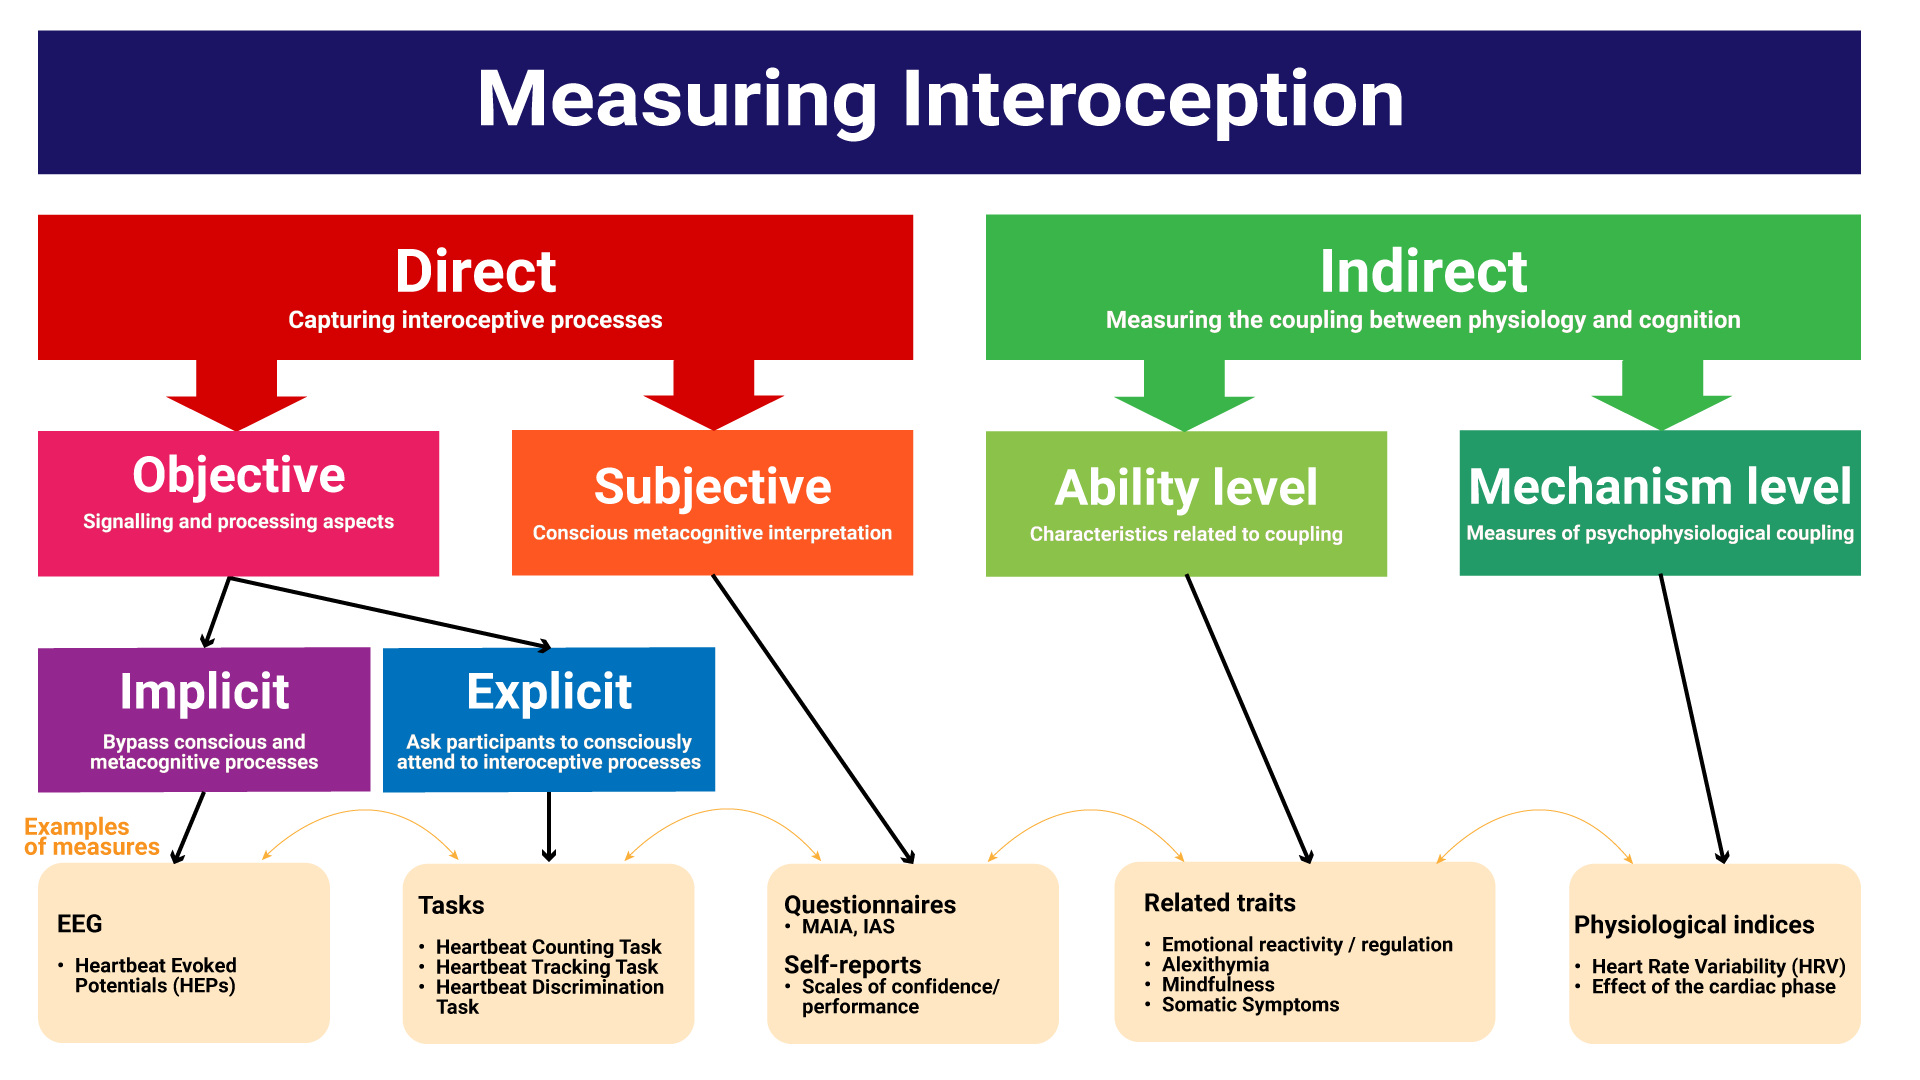
\includegraphics[width=1\linewidth,height=\textheight,keepaspectratio]{figures/MeasuringInteroception.png}

\end{figure*}

Although the use of subjective self-report questionnaires to measure
deeply embodied functions might seem paradoxical at first, recent
redefinitions of interoception emphasize the role of high-level and
metacognitive elaboration of interoceptive information. These
redefinitions provide theoretical grounding to support the idea that
some facets of interoception, including participants' metacognitive
beliefs, can be assessed subjectively
(\citeproc{ref-khalsa2018interoception}{Khalsa et al., 2018};
\citeproc{ref-suksasilp2022towards}{Suksasilp \& Garfinkel, 2022}).
Moreover, the notion that self-reports might not reflect the same
processes as other interoception tasks might be important to
contextualize the apparent lack of convergence between measures in the
field (\citeproc{ref-desmedt2022measures}{Desmedt et al., 2022}). For
instance, existing findings typically show weak or no correlations
between questionnaires and objective measures, such as the Heartbeat
Counting Task (HCT, \citeproc{ref-schandry1981heart}{Schandry, 1981})
and the Heartbeat Detection Task (HDT,
\citeproc{ref-kleckner2015methodological}{Kleckner et al., 2015}),
including for measures of the same theoretical dimensions
(\citeproc{ref-arslanova2022}{Arslanova et al., 2022};
\citeproc{ref-brand2023}{Brand et al., 2023}; e.g., task-based accuracy
vs.~self-reported accuracy, \citeproc{ref-murphy2019}{Murphy et al.,
2019}). Additionally, even various objective measures assessing in
theory the same interoceptive dimension, such as accuracy, either show
no or weak correlation (respectively, \citeproc{ref-brand2023}{Brand et
al., 2023}; \citeproc{ref-hickman2020relationship}{Hickman et al.,
2020}). Perhaps more surprisingly, low correlations have been observed
even among questionnaires, suggesting (in parallel to major validity
concerns) the potential targeting of different facets related to
interoception.

One striking example concerns the assessment of interoceptive
sensibility, which is broadly defined as the self-reported tendency to
focus on and detect internal sensations
(\citeproc{ref-garfinkel2015knowing}{Garfinkel et al., 2015}), but more
narrowly as the subjective tendency to focus on interoceptive signals,
without necessarily implying detection ability
(\citeproc{ref-khalsa2018interoception}{Khalsa et al., 2018}). A recent
systematic review suggested that various questionnaires designed to
assess interoceptive sensibility may, in fact, measure distinct
constructs, with the risk of researchers treating them as equivalent
despite overall low convergence
(\citeproc{ref-desmedt2022measures}{Desmedt et al., 2022}). Notably,
this review adopted a broad definition of sensibility, incorporating
both interoceptive sensibility and interoceptive self-report scales,
following the eight-facet model by Khalsa et al.
(\citeproc{ref-khalsa2018interoception}{2018}). Several widely used
questionnaires were included in the review, such as the Multidimensional
Assessment of Interoceptive Awareness (MAIA,
\citeproc{ref-mehling2012}{Mehling et al., 2012}; MAIA-2,
\citeproc{ref-mehling2018multidimensional}{Mehling et al., 2018}), the
Body Perception Questionnaire (BPQ,
\citeproc{ref-porges1993body}{Porges, 1993}), the Private subscale of
the Body Consciousness Questionnaire (PBCS,
\citeproc{ref-miller1981consciousness}{Miller et al., 1981}), the Body
Awareness Questionnaire (BAQ, \citeproc{ref-shields1989body}{Shields et
al., 1989}), and the Eating Disorder Inventory
(\citeproc{ref-garner1983}{Garner et al., 1983}; EDI,
\citeproc{ref-garner1991eating}{Garner, 1991}). The lack of correlations
to moderate correlations among these questionnaires highlight the need
for greater conceptual clarity regarding what each measure captures, how
they relate to different dimensions of interoception, and their
potential overlaps with other constructs, such as alexithymia and body
awareness.

\subsection{The Interoceptive Accuracy Scale
(IAS)}\label{the-interoceptive-accuracy-scale-ias}

Focusing on another dimension of interoception, a recently developed
scale with a rapidly growing popularity is the Interoceptive Accuracy
Scale (IAS, \citeproc{ref-murphy2019}{Murphy et al., 2019}). The IAS
consists of 21 Likert-scale items that query how accurately one can
perceive different bodily signals, with one item per physiological
modality such as respiration (\emph{``I can always accurately perceive
when I am breathing fast''}), heart (\emph{``I can always accurately
perceive when my heart is beating fast''}), skin (\emph{``I can always
accurately perceive when something is going to be ticklish''}), arousal
or bodily functions like coughing (\emph{``I can always accurately
perceive when I am going to cough''}) or urinating (\emph{``I can always
accurately perceive when I need to urinate''}). Appealingly, the IAS'
statements are about specific interoceptive behaviours, which is a
distinct difference with other popular interoception questionnaires,
such as the MAIA-2, which contains more general and metacognitive items
(e.g., \emph{``I trust my body sensations''}, \emph{``I can notice an
unpleasant body sensation without worrying about it''}), as well as
dimensions related to attention regulation (e.g., Not-distracting) or
emotion regulation (e.g., Not-worrying).

{[}\textbf{NOTES}: todd 2022 found no correlation for MAIA and IAS
except with the non-worrying facet + Gaggero found positive correlations
with IAS and MAIA (general){]}

The original validation study suggested a two-factor structure for the
IAS, one reflecting the perception of general interoceptive signals
(urinate, hungry, defecate, thirsty, pain, heart, taste, breathing,
temperature, muscles, affective touch, vomit, sexual arousal), and other
relating to signals that may be difficult to perceive solely through
interoceptive information (itch, tickle, cough, burp, bruise, blood
sugar, sneeze, wind). The authors however underlined its acceptable but
imperfect fit (\citeproc{ref-murphy2019}{Murphy et al., 2019, p. 127}),
and several follow-up studies have indeed identified different optimal
solutions. For instance, Brand et al. (\citeproc{ref-brand2023}{2023})
reported a 1-factor solution, while Lin et al.
(\citeproc{ref-lin2023}{2023}) - using Exploratory Graph Analysis (EGA,
\citeproc{ref-golino2017exploratory}{H. F. Golino \& Epskamp, 2017}) -
and Campos et al. (\citeproc{ref-campos2021}{2021}) found bifactor
solutions (i.e., one general factor above a set of lower-level factors,
\citeproc{ref-rodriguez2016evaluating}{Rodriguez et al., 2016}) to be
the best fit. Using a 2-factors Exploratory Factor Analysis (EFA), Koike
and Nomura (\citeproc{ref-koike2023}{2023}) suggested that the items
could be grouped into cutaneous (itching, tickling, coughing, burping,
affective touch, bruising, passing gas, sneezing, muscle sensations,
sexual arousal, and taste) and visceral sensations (urination,
defecation, hunger, thirst, pain, breathing, fatigue/blood sugar,
temperature, vomiting, and heartbeat).

Discussions have also been focused on specific items. For instance,
Murphy et al. (\citeproc{ref-murphy2019}{2019}) notes that some items
might measure direct interoceptive signals such as cardioception, while
others might capture phenomena not perceivable through interoceptive
signals alone (e.g., ``bruising''; p.~119). Lin et al.
(\citeproc{ref-lin2023}{2023}) additionally highlights five locally
dependent pairs and three items (touch, blood sugar, bruise) with
exceptionally high difficulty and low discrimination, and Campos et al.
(\citeproc{ref-campos2021}{2021}) reported ``tickle'' to be the only
item that reflected more specific factors than the general factor.
Furthermore, localization issues also arose, with both ``itch'' and
``tickle'' corresponding to the same Chinese character, leading to their
collapse into a single item (\citeproc{ref-lin2023}{Lin et al., 2023}).

Regarding its validity, the IAS has naturally been compared to other
interoception-related measures, and shows a positive correlations with
most facets of the MAIA
(\citeproc{ref-mehling2018multidimensional}{Mehling et al., 2018}),
except for the Not-Distracting and Not-Worrying subscales
(\citeproc{ref-brand2023}{Brand et al., 2023}) - which were previously
highlighted as related to non-interoceptive abilities
(\citeproc{ref-ferentzi2021examining}{Ferentzi et al., 2021}).
Interestingly, findings on the correlation between the IAS and the body
awareness dimension of the BPQ (i.e., BPQ-A) have been mixed: some
studies report small positive correlations
(\citeproc{ref-brand2023}{Brand et al., 2023};
\citeproc{ref-campos2021}{Campos et al., 2021};
\citeproc{ref-koike2023}{Koike \& Nomura, 2023}), while others find
small negative correlations (\citeproc{ref-lin2023}{Lin et al., 2023})
or no correlation at all (\citeproc{ref-murphy2019}{Murphy et al.,
2019}). Small positive correlations have also been observed with the
``observation'' and ``description'' subscales of the Five Facet
Mindfulness Questionnaire (FFMQ, \citeproc{ref-baer2006using}{Baer et
al., 2006}; \citeproc{ref-brand2023}{Brand et al., 2023};
\citeproc{ref-koike2023}{Koike \& Nomura, 2023}), as well as with the
``non-reactivity'' and ``acting with awareness'' subscales
(\citeproc{ref-koike2023}{Koike \& Nomura, 2023}). Additionally, the IAS
has shown a positive correlation with the interoceptive awareness
subscale of the Eating Disorder Inventory (EDI-IA,
\citeproc{ref-lin2023}{Lin et al., 2023}) and a negative correlation
with the Interoceptive Confusion Questionnaire (ICQ,
\citeproc{ref-brewer2016alexithymia}{Brewer et al., 2016}), as reported
by Brand et al. (\citeproc{ref-brand2023}{2023}) and Murphy et al.
(\citeproc{ref-murphy2019}{2019}). Lastly, the correlation with the
Interoceptive Attention Scale (IATS,
\citeproc{ref-gabriele2022dissociations}{Gabriele et al., 2022}) appears
rather small (\citeproc{ref-koike2023}{Koike \& Nomura, 2023};
\citeproc{ref-lin2023}{Lin et al., 2023}).

While assessing the predictive validity of an interoception scale can be
conceived as theoretically challenging, expected negative associations
were observed between the IAS and alexithymia
(\citeproc{ref-brand2023}{Brand et al., 2023};
\citeproc{ref-campos2021}{Campos et al., 2021};
\citeproc{ref-koike2023}{Koike \& Nomura, 2023};
\citeproc{ref-lin2023}{Lin et al., 2023};
\citeproc{ref-murphy2019}{Murphy et al., 2019}), somatic symptoms
(\citeproc{ref-brand2023}{Brand et al., 2023};
\citeproc{ref-koike2023}{Koike \& Nomura, 2023};
\citeproc{ref-lin2023}{Lin et al., 2023}), depressive symptoms
(\citeproc{ref-brand2023}{Brand et al., 2023};
\citeproc{ref-koike2023}{Koike \& Nomura, 2023};
\citeproc{ref-lin2023}{Lin et al., 2023}), anxiety
(\citeproc{ref-brand2023}{Brand et al., 2023}), neuroticism
(\citeproc{ref-brand2023}{Brand et al., 2023}) and self-esteem
(\citeproc{ref-murphy2019}{Murphy et al., 2019}). Taken together, these
findings support the IAS as measuring an adaptive aspect of
interoception, although its pattern of associations with other
interoception (or interoception-related) questionnaires points towards
some overlap across various theoretical dimensions, casting some doubt
on the orthogonal models of interoception and the possibility of its
faithful capture by questionnaires.

The current study aims at 1) clarifying the structure of the IAS with a
mega-analytic (which involves a re-analysis at the raw data level by
aggregating datasets) approach that leverages existing data and contrast
the traditional CFA/SEM factor-based analyses with network-based ones
(Exploratory Graph Analysis); 1) provide an overview of the
dispositional correlates of the IAS, clarifying its general pattern of
associations, which is key to better understand the nature, place and
role of interoception questionnaires within a larger context.

\section{Study 1}\label{study-1}

Study 1 will re-analyse and assess the factor structure of the IAS by
taking advantage of the large number of open-access datasets
(\citeproc{ref-arslanova2022}{Arslanova et al., 2022};
\citeproc{ref-brand2022}{Brand et al., 2022};
\citeproc{ref-brand2023}{Brand et al., 2023};
\citeproc{ref-campos2021}{Campos et al., 2021};
\citeproc{ref-gaggero2021}{Gaggero et al., 2021};
\citeproc{ref-lin2023}{Lin et al., 2023};
\citeproc{ref-makowski2025measuring}{Makowski et al., 2025};
\citeproc{ref-murphy2019}{Murphy et al., 2019};
\citeproc{ref-poerio2024interoceptive}{Poerio et al., 2024};
\citeproc{ref-todd2022}{Todd et al., 2022}; \citeproc{ref-von2023}{Von
Mohr et al., 2023}). While combining these studies might provide a more
robust and generalizable understanding of the IAS' factor structure, we
also additionally provide an individual analysis (i.e., applying the
same method on all samples separately) to add nuance to the general
picture, as all studies differ in their sample size, demographic
characteristics, language, and procedure.

\subsection{Methods}\label{methods}

\subsubsection{Datasets}\label{datasets}

Our search focused on studies citing the original IAS validation paper
(\citeproc{ref-murphy2019}{Murphy et al., 2019}), identifying 136 papers
(as of 01/05/2024). To qualify for inclusion, papers needed to (1)
provide accessible data in open-access, (2) employ the IAS as a measure,
and (3) report individual IAS items scores. We also included the data of
five unpublished studies. A total of 16 datasets was included (see
\textbf{Table 1}).

The total number of participants was 33,272 participants (Mean = 48.09
\(\pm\) 13.1, 71.3\% Female).

\begin{twocolumntable}

\global\setlength{\Oldarrayrulewidth}{\arrayrulewidth}

\global\setlength{\Oldtabcolsep}{\tabcolsep}

\setlength{\tabcolsep}{2pt}

\renewcommand*{\arraystretch}{1}



\providecommand{\ascline}[3]{\noalign{\global\arrayrulewidth #1}\arrayrulecolor[HTML]{#2}\cline{#3}}

\begin{longtable}[c]{ccccccccc}

\caption{\label{tbl-table1}Description of the samples used in the
study.}

\tabularnewline

\ascline{0.75pt}{000000}{1-9}

\multicolumn{1}{>{}c}{\textcolor[HTML]{000000}{\fontsize{6}{12}\selectfont{\global\setmainfont{Times New Roman}{Sample}}}} & \multicolumn{1}{>{}c}{\textcolor[HTML]{000000}{\fontsize{6}{12}\selectfont{\global\setmainfont{Times New Roman}{Reference}}}} & \multicolumn{1}{>{}c}{\textcolor[HTML]{000000}{\fontsize{6}{12}\selectfont{\global\setmainfont{Times New Roman}{Language}}}} & \multicolumn{1}{>{}c}{\textcolor[HTML]{000000}{\fontsize{6}{12}\selectfont{\global\setmainfont{Times New Roman}{N}}}} & \multicolumn{1}{>{}c}{\textcolor[HTML]{000000}{\fontsize{6}{12}\selectfont{\global\setmainfont{Times New Roman}{Difference}}}} & \multicolumn{1}{>{}c}{\textcolor[HTML]{000000}{\fontsize{6}{12}\selectfont{\global\setmainfont{Times New Roman}{Age\ (Mean\ \ ±\ SD)}}}} & \multicolumn{1}{>{}c}{\textcolor[HTML]{000000}{\fontsize{6}{12}\selectfont{\global\setmainfont{Times New Roman}{Range}}}} & \multicolumn{1}{>{}c}{\textcolor[HTML]{000000}{\fontsize{6}{12}\selectfont{\global\setmainfont{Times New Roman}{Female\ \%}}}} & \multicolumn{1}{>{}c}{\textcolor[HTML]{000000}{\fontsize{6}{12}\selectfont{\global\setmainfont{Times New Roman}{Availability}}}} \\

\ascline{0.75pt}{000000}{1-9}\endfirsthead 

\ascline{0.75pt}{000000}{1-9}

\multicolumn{1}{>{}c}{\textcolor[HTML]{000000}{\fontsize{6}{12}\selectfont{\global\setmainfont{Times New Roman}{Sample}}}} & \multicolumn{1}{>{}c}{\textcolor[HTML]{000000}{\fontsize{6}{12}\selectfont{\global\setmainfont{Times New Roman}{Reference}}}} & \multicolumn{1}{>{}c}{\textcolor[HTML]{000000}{\fontsize{6}{12}\selectfont{\global\setmainfont{Times New Roman}{Language}}}} & \multicolumn{1}{>{}c}{\textcolor[HTML]{000000}{\fontsize{6}{12}\selectfont{\global\setmainfont{Times New Roman}{N}}}} & \multicolumn{1}{>{}c}{\textcolor[HTML]{000000}{\fontsize{6}{12}\selectfont{\global\setmainfont{Times New Roman}{Difference}}}} & \multicolumn{1}{>{}c}{\textcolor[HTML]{000000}{\fontsize{6}{12}\selectfont{\global\setmainfont{Times New Roman}{Age\ (Mean\ \ ±\ SD)}}}} & \multicolumn{1}{>{}c}{\textcolor[HTML]{000000}{\fontsize{6}{12}\selectfont{\global\setmainfont{Times New Roman}{Range}}}} & \multicolumn{1}{>{}c}{\textcolor[HTML]{000000}{\fontsize{6}{12}\selectfont{\global\setmainfont{Times New Roman}{Female\ \%}}}} & \multicolumn{1}{>{}c}{\textcolor[HTML]{000000}{\fontsize{6}{12}\selectfont{\global\setmainfont{Times New Roman}{Availability}}}} \\

\ascline{0.75pt}{000000}{1-9}\endhead



\multicolumn{1}{>{}c}{\textcolor[HTML]{000000}{\fontsize{6}{12}\selectfont{\global\setmainfont{Times New Roman}{}}}} & \multicolumn{1}{>{}c}{\textcolor[HTML]{000000}{\fontsize{6}{12}\selectfont{\global\setmainfont{Times New Roman}{Murphy\ et\ al.,\ (2020)}}}} & \multicolumn{1}{>{}c}{\textcolor[HTML]{000000}{\fontsize{6}{12}\selectfont{\global\setmainfont{Times New Roman}{}}}} & \multicolumn{1}{>{}c}{\textcolor[HTML]{000000}{\fontsize{6}{12}\selectfont{\global\setmainfont{Times New Roman}{}}}} & \multicolumn{1}{>{}c}{\textcolor[HTML]{000000}{\fontsize{6}{12}\selectfont{\global\setmainfont{Times New Roman}{}}}} & \multicolumn{1}{>{}c}{\textcolor[HTML]{000000}{\fontsize{6}{12}\selectfont{\global\setmainfont{Times New Roman}{}}}} & \multicolumn{1}{>{}c}{\textcolor[HTML]{000000}{\fontsize{6}{12}\selectfont{\global\setmainfont{Times New Roman}{}}}} & \multicolumn{1}{>{}c}{\textcolor[HTML]{000000}{\fontsize{6}{12}\selectfont{\global\setmainfont{Times New Roman}{}}}} & \multicolumn{1}{>{}c}{\textcolor[HTML]{000000}{\fontsize{6}{12}\selectfont{\global\setmainfont{Times New Roman}{osf.io/3m5nh}}}} \\





\multicolumn{1}{>{}c}{\textcolor[HTML]{000000}{\fontsize{6}{12}\selectfont{\global\setmainfont{Times New Roman}{Sample\ 1a}}}} & \multicolumn{1}{>{}c}{\textcolor[HTML]{000000}{\fontsize{6}{12}\selectfont{\global\setmainfont{Times New Roman}{}}}} & \multicolumn{1}{>{}c}{\textcolor[HTML]{000000}{\fontsize{6}{12}\selectfont{\global\setmainfont{Times New Roman}{English}}}} & \multicolumn{1}{>{}c}{\textcolor[HTML]{000000}{\fontsize{6}{12}\selectfont{\global\setmainfont{Times New Roman}{451}}}} & \multicolumn{1}{>{}c}{\textcolor[HTML]{000000}{\fontsize{6}{12}\selectfont{\global\setmainfont{Times New Roman}{}}}} & \multicolumn{1}{>{}c}{\textcolor[HTML]{000000}{\fontsize{6}{12}\selectfont{\global\setmainfont{Times New Roman}{25.8\ ±\ 8.4}}}} & \multicolumn{1}{>{}c}{\textcolor[HTML]{000000}{\fontsize{6}{12}\selectfont{\global\setmainfont{Times New Roman}{18-69}}}} & \multicolumn{1}{>{}c}{\textcolor[HTML]{000000}{\fontsize{6}{12}\selectfont{\global\setmainfont{Times New Roman}{69.4\%}}}} & \multicolumn{1}{>{}c}{\textcolor[HTML]{000000}{\fontsize{6}{12}\selectfont{\global\setmainfont{Times New Roman}{}}}} \\





\multicolumn{1}{>{}c}{\textcolor[HTML]{000000}{\fontsize{6}{12}\selectfont{\global\setmainfont{Times New Roman}{Sample\ 1b}}}} & \multicolumn{1}{>{}c}{\textcolor[HTML]{000000}{\fontsize{6}{12}\selectfont{\global\setmainfont{Times New Roman}{}}}} & \multicolumn{1}{>{}c}{\textcolor[HTML]{000000}{\fontsize{6}{12}\selectfont{\global\setmainfont{Times New Roman}{English}}}} & \multicolumn{1}{>{}c}{\textcolor[HTML]{000000}{\fontsize{6}{12}\selectfont{\global\setmainfont{Times New Roman}{375}}}} & \multicolumn{1}{>{}c}{\textcolor[HTML]{000000}{\fontsize{6}{12}\selectfont{\global\setmainfont{Times New Roman}{}}}} & \multicolumn{1}{>{}c}{\textcolor[HTML]{000000}{\fontsize{6}{12}\selectfont{\global\setmainfont{Times New Roman}{35.3\ ±\ 16.9}}}} & \multicolumn{1}{>{}c}{\textcolor[HTML]{000000}{\fontsize{6}{12}\selectfont{\global\setmainfont{Times New Roman}{18-91}}}} & \multicolumn{1}{>{}c}{\textcolor[HTML]{000000}{\fontsize{6}{12}\selectfont{\global\setmainfont{Times New Roman}{70.1\%}}}} & \multicolumn{1}{>{}c}{\textcolor[HTML]{000000}{\fontsize{6}{12}\selectfont{\global\setmainfont{Times New Roman}{}}}} \\





\multicolumn{1}{>{}c}{\textcolor[HTML]{000000}{\fontsize{6}{12}\selectfont{\global\setmainfont{Times New Roman}{Sample\ 2}}}} & \multicolumn{1}{>{}c}{\textcolor[HTML]{000000}{\fontsize{6}{12}\selectfont{\global\setmainfont{Times New Roman}{Gaggero\ et\ al.,\ (2021)}}}} & \multicolumn{1}{>{}c}{\textcolor[HTML]{000000}{\fontsize{6}{12}\selectfont{\global\setmainfont{Times New Roman}{English\ and\ Italian}}}} & \multicolumn{1}{>{}c}{\textcolor[HTML]{000000}{\fontsize{6}{12}\selectfont{\global\setmainfont{Times New Roman}{814}}}} & \multicolumn{1}{>{}c}{\textcolor[HTML]{000000}{\fontsize{6}{12}\selectfont{\global\setmainfont{Times New Roman}{}}}} & \multicolumn{1}{>{}c}{\textcolor[HTML]{000000}{\fontsize{6}{12}\selectfont{\global\setmainfont{Times New Roman}{24.9\ ±\ 5.3}}}} & \multicolumn{1}{>{}c}{\textcolor[HTML]{000000}{\fontsize{6}{12}\selectfont{\global\setmainfont{Times New Roman}{18-58}}}} & \multicolumn{1}{>{}c}{\textcolor[HTML]{000000}{\fontsize{6}{12}\selectfont{\global\setmainfont{Times New Roman}{60.3\%}}}} & \multicolumn{1}{>{}c}{\textcolor[HTML]{000000}{\fontsize{6}{12}\selectfont{\global\setmainfont{Times New Roman}{osf.io/5x9sg}}}} \\





\multicolumn{1}{>{}c}{\textcolor[HTML]{000000}{\fontsize{6}{12}\selectfont{\global\setmainfont{Times New Roman}{Sample\ 3}}}} & \multicolumn{1}{>{}c}{\textcolor[HTML]{000000}{\fontsize{6}{12}\selectfont{\global\setmainfont{Times New Roman}{Campos\ et\ al.,\ (2022)}}}} & \multicolumn{1}{>{}c}{\textcolor[HTML]{000000}{\fontsize{6}{12}\selectfont{\global\setmainfont{Times New Roman}{Portuguese}}}} & \multicolumn{1}{>{}c}{\textcolor[HTML]{000000}{\fontsize{6}{12}\selectfont{\global\setmainfont{Times New Roman}{515}}}} & \multicolumn{1}{>{}c}{\textcolor[HTML]{000000}{\fontsize{6}{12}\selectfont{\global\setmainfont{Times New Roman}{}}}} & \multicolumn{1}{>{}c}{\textcolor[HTML]{000000}{\fontsize{6}{12}\selectfont{\global\setmainfont{Times New Roman}{30.7\ ±\ 10.5}}}} & \multicolumn{1}{>{}c}{\textcolor[HTML]{000000}{\fontsize{6}{12}\selectfont{\global\setmainfont{Times New Roman}{18-72}}}} & \multicolumn{1}{>{}c}{\textcolor[HTML]{000000}{\fontsize{6}{12}\selectfont{\global\setmainfont{Times New Roman}{59.6\%}}}} & \multicolumn{1}{>{}c}{\textcolor[HTML]{000000}{\fontsize{6}{12}\selectfont{\global\setmainfont{Times New Roman}{osf.io/j6ef3}}}} \\





\multicolumn{1}{>{}c}{\textcolor[HTML]{000000}{\fontsize{6}{12}\selectfont{\global\setmainfont{Times New Roman}{Sample\ 4}}}} & \multicolumn{1}{>{}c}{\textcolor[HTML]{000000}{\fontsize{6}{12}\selectfont{\global\setmainfont{Times New Roman}{Todd\ et\ al.,\ (2022)}}}} & \multicolumn{1}{>{}c}{\textcolor[HTML]{000000}{\fontsize{6}{12}\selectfont{\global\setmainfont{Times New Roman}{English}}}} & \multicolumn{1}{>{}c}{\textcolor[HTML]{000000}{\fontsize{6}{12}\selectfont{\global\setmainfont{Times New Roman}{802}}}} & \multicolumn{1}{>{}c}{\textcolor[HTML]{000000}{\fontsize{6}{12}\selectfont{\global\setmainfont{Times New Roman}{}}}} & \multicolumn{1}{>{}c}{\textcolor[HTML]{000000}{\fontsize{6}{12}\selectfont{\global\setmainfont{Times New Roman}{48.6.6\ ±\ 14.1*}}}} & \multicolumn{1}{>{}c}{\textcolor[HTML]{000000}{\fontsize{6}{12}\selectfont{\global\setmainfont{Times New Roman}{18-92*}}}} & \multicolumn{1}{>{}c}{\textcolor[HTML]{000000}{\fontsize{6}{12}\selectfont{\global\setmainfont{Times New Roman}{50\%*}}}} & \multicolumn{1}{>{}c}{\textcolor[HTML]{000000}{\fontsize{6}{12}\selectfont{\global\setmainfont{Times New Roman}{osf.io/ms354}}}} \\





\multicolumn{1}{>{}c}{\textcolor[HTML]{000000}{\fontsize{6}{12}\selectfont{\global\setmainfont{Times New Roman}{Sample\ 5}}}} & \multicolumn{1}{>{}c}{\textcolor[HTML]{000000}{\fontsize{6}{12}\selectfont{\global\setmainfont{Times New Roman}{Arslanova\ et\ al.,\ (2022)}}}} & \multicolumn{1}{>{}c}{\textcolor[HTML]{000000}{\fontsize{6}{12}\selectfont{\global\setmainfont{Times New Roman}{English}}}} & \multicolumn{1}{>{}c}{\textcolor[HTML]{000000}{\fontsize{6}{12}\selectfont{\global\setmainfont{Times New Roman}{143}}}} & \multicolumn{1}{>{}c}{\textcolor[HTML]{000000}{\fontsize{6}{12}\selectfont{\global\setmainfont{Times New Roman}{}}}} & \multicolumn{1}{>{}c}{\textcolor[HTML]{000000}{\fontsize{6}{12}\selectfont{\global\setmainfont{Times New Roman}{28.5\ ±\ 7.6}}}} & \multicolumn{1}{>{}c}{\textcolor[HTML]{000000}{\fontsize{6}{12}\selectfont{\global\setmainfont{Times New Roman}{18-73}}}} & \multicolumn{1}{>{}c}{\textcolor[HTML]{000000}{\fontsize{6}{12}\selectfont{\global\setmainfont{Times New Roman}{46.8\%}}}} & \multicolumn{1}{>{}c}{\textcolor[HTML]{000000}{\fontsize{6}{12}\selectfont{\global\setmainfont{Times New Roman}{osf.io/mp3cy}}}} \\





\multicolumn{1}{>{}c}{\textcolor[HTML]{000000}{\fontsize{6}{12}\selectfont{\global\setmainfont{Times New Roman}{Sample\ 6}}}} & \multicolumn{1}{>{}c}{\textcolor[HTML]{000000}{\fontsize{6}{12}\selectfont{\global\setmainfont{Times New Roman}{Brand\ et\ al.,\ (2022)}}}} & \multicolumn{1}{>{}c}{\textcolor[HTML]{000000}{\fontsize{6}{12}\selectfont{\global\setmainfont{Times New Roman}{German}}}} & \multicolumn{1}{>{}c}{\textcolor[HTML]{000000}{\fontsize{6}{12}\selectfont{\global\setmainfont{Times New Roman}{619}}}} & \multicolumn{1}{>{}c}{\textcolor[HTML]{000000}{\fontsize{6}{12}\selectfont{\global\setmainfont{Times New Roman}{}}}} & \multicolumn{1}{>{}c}{\textcolor[HTML]{000000}{\fontsize{6}{12}\selectfont{\global\setmainfont{Times New Roman}{43.9\ ±\ 14.5}}}} & \multicolumn{1}{>{}c}{\textcolor[HTML]{000000}{\fontsize{6}{12}\selectfont{\global\setmainfont{Times New Roman}{18-78}}}} & \multicolumn{1}{>{}c}{\textcolor[HTML]{000000}{\fontsize{6}{12}\selectfont{\global\setmainfont{Times New Roman}{78.7\%}}}} & \multicolumn{1}{>{}c}{\textcolor[HTML]{000000}{\fontsize{6}{12}\selectfont{\global\setmainfont{Times New Roman}{osf.io/xwz6g}}}} \\





\multicolumn{1}{>{}c}{\textcolor[HTML]{000000}{\fontsize{6}{12}\selectfont{\global\setmainfont{Times New Roman}{}}}} & \multicolumn{1}{>{}c}{\textcolor[HTML]{000000}{\fontsize{6}{12}\selectfont{\global\setmainfont{Times New Roman}{Brand\ et\ al.,\ (2023)}}}} & \multicolumn{1}{>{}c}{\textcolor[HTML]{000000}{\fontsize{6}{12}\selectfont{\global\setmainfont{Times New Roman}{}}}} & \multicolumn{1}{>{}c}{\textcolor[HTML]{000000}{\fontsize{6}{12}\selectfont{\global\setmainfont{Times New Roman}{}}}} & \multicolumn{1}{>{}c}{\textcolor[HTML]{000000}{\fontsize{6}{12}\selectfont{\global\setmainfont{Times New Roman}{}}}} & \multicolumn{1}{>{}c}{\textcolor[HTML]{000000}{\fontsize{6}{12}\selectfont{\global\setmainfont{Times New Roman}{}}}} & \multicolumn{1}{>{}c}{\textcolor[HTML]{000000}{\fontsize{6}{12}\selectfont{\global\setmainfont{Times New Roman}{}}}} & \multicolumn{1}{>{}c}{\textcolor[HTML]{000000}{\fontsize{6}{12}\selectfont{\global\setmainfont{Times New Roman}{}}}} & \multicolumn{1}{>{}c}{\textcolor[HTML]{000000}{\fontsize{6}{12}\selectfont{\global\setmainfont{Times New Roman}{osf.io/3f2h6}}}} \\





\multicolumn{1}{>{}c}{\textcolor[HTML]{000000}{\fontsize{6}{12}\selectfont{\global\setmainfont{Times New Roman}{Sample\ 7a}}}} & \multicolumn{1}{>{}c}{\textcolor[HTML]{000000}{\fontsize{6}{12}\selectfont{\global\setmainfont{Times New Roman}{}}}} & \multicolumn{1}{>{}c}{\textcolor[HTML]{000000}{\fontsize{6}{12}\selectfont{\global\setmainfont{Times New Roman}{German}}}} & \multicolumn{1}{>{}c}{\textcolor[HTML]{000000}{\fontsize{6}{12}\selectfont{\global\setmainfont{Times New Roman}{522}}}} & \multicolumn{1}{>{}c}{\textcolor[HTML]{000000}{\fontsize{6}{12}\selectfont{\global\setmainfont{Times New Roman}{}}}} & \multicolumn{1}{>{}c}{\textcolor[HTML]{000000}{\fontsize{6}{12}\selectfont{\global\setmainfont{Times New Roman}{23.4\ ±\ 6.7}}}} & \multicolumn{1}{>{}c}{\textcolor[HTML]{000000}{\fontsize{6}{12}\selectfont{\global\setmainfont{Times New Roman}{18-79}}}} & \multicolumn{1}{>{}c}{\textcolor[HTML]{000000}{\fontsize{6}{12}\selectfont{\global\setmainfont{Times New Roman}{79.5\%}}}} & \multicolumn{1}{>{}c}{\textcolor[HTML]{000000}{\fontsize{6}{12}\selectfont{\global\setmainfont{Times New Roman}{}}}} \\





\multicolumn{1}{>{}c}{\textcolor[HTML]{000000}{\fontsize{6}{12}\selectfont{\global\setmainfont{Times New Roman}{Sample\ 7b}}}} & \multicolumn{1}{>{}c}{\textcolor[HTML]{000000}{\fontsize{6}{12}\selectfont{\global\setmainfont{Times New Roman}{}}}} & \multicolumn{1}{>{}c}{\textcolor[HTML]{000000}{\fontsize{6}{12}\selectfont{\global\setmainfont{Times New Roman}{German}}}} & \multicolumn{1}{>{}c}{\textcolor[HTML]{000000}{\fontsize{6}{12}\selectfont{\global\setmainfont{Times New Roman}{1993}}}} & \multicolumn{1}{>{}c}{\textcolor[HTML]{000000}{\fontsize{6}{12}\selectfont{\global\setmainfont{Times New Roman}{}}}} & \multicolumn{1}{>{}c}{\textcolor[HTML]{000000}{\fontsize{6}{12}\selectfont{\global\setmainfont{Times New Roman}{32.0\ ±\ 12.6}}}} & \multicolumn{1}{>{}c}{\textcolor[HTML]{000000}{\fontsize{6}{12}\selectfont{\global\setmainfont{Times New Roman}{16-81}}}} & \multicolumn{1}{>{}c}{\textcolor[HTML]{000000}{\fontsize{6}{12}\selectfont{\global\setmainfont{Times New Roman}{77.7\%}}}} & \multicolumn{1}{>{}c}{\textcolor[HTML]{000000}{\fontsize{6}{12}\selectfont{\global\setmainfont{Times New Roman}{}}}} \\





\multicolumn{1}{>{}c}{\textcolor[HTML]{000000}{\fontsize{6}{12}\selectfont{\global\setmainfont{Times New Roman}{Sample\ 7c}}}} & \multicolumn{1}{>{}c}{\textcolor[HTML]{000000}{\fontsize{6}{12}\selectfont{\global\setmainfont{Times New Roman}{}}}} & \multicolumn{1}{>{}c}{\textcolor[HTML]{000000}{\fontsize{6}{12}\selectfont{\global\setmainfont{Times New Roman}{German}}}} & \multicolumn{1}{>{}c}{\textcolor[HTML]{000000}{\fontsize{6}{12}\selectfont{\global\setmainfont{Times New Roman}{802}}}} & \multicolumn{1}{>{}c}{\textcolor[HTML]{000000}{\fontsize{6}{12}\selectfont{\global\setmainfont{Times New Roman}{}}}} & \multicolumn{1}{>{}c}{\textcolor[HTML]{000000}{\fontsize{6}{12}\selectfont{\global\setmainfont{Times New Roman}{27.3\ ±\ 9.3}}}} & \multicolumn{1}{>{}c}{\textcolor[HTML]{000000}{\fontsize{6}{12}\selectfont{\global\setmainfont{Times New Roman}{18-72}}}} & \multicolumn{1}{>{}c}{\textcolor[HTML]{000000}{\fontsize{6}{12}\selectfont{\global\setmainfont{Times New Roman}{68.9\%}}}} & \multicolumn{1}{>{}c}{\textcolor[HTML]{000000}{\fontsize{6}{12}\selectfont{\global\setmainfont{Times New Roman}{}}}} \\





\multicolumn{1}{>{}c}{\textcolor[HTML]{000000}{\fontsize{6}{12}\selectfont{\global\setmainfont{Times New Roman}{}}}} & \multicolumn{1}{>{}c}{\textcolor[HTML]{000000}{\fontsize{6}{12}\selectfont{\global\setmainfont{Times New Roman}{Lin\ et\ al.,\ (2023)}}}} & \multicolumn{1}{>{}c}{\textcolor[HTML]{000000}{\fontsize{6}{12}\selectfont{\global\setmainfont{Times New Roman}{}}}} & \multicolumn{1}{>{}c}{\textcolor[HTML]{000000}{\fontsize{6}{12}\selectfont{\global\setmainfont{Times New Roman}{}}}} & \multicolumn{1}{>{}c}{\textcolor[HTML]{000000}{\fontsize{6}{12}\selectfont{\global\setmainfont{Times New Roman}{}}}} & \multicolumn{1}{>{}c}{\textcolor[HTML]{000000}{\fontsize{6}{12}\selectfont{\global\setmainfont{Times New Roman}{}}}} & \multicolumn{1}{>{}c}{\textcolor[HTML]{000000}{\fontsize{6}{12}\selectfont{\global\setmainfont{Times New Roman}{}}}} & \multicolumn{1}{>{}c}{\textcolor[HTML]{000000}{\fontsize{6}{12}\selectfont{\global\setmainfont{Times New Roman}{}}}} & \multicolumn{1}{>{}c}{\textcolor[HTML]{000000}{\fontsize{6}{12}\selectfont{\global\setmainfont{Times New Roman}{osf.io/3eztd}}}} \\





\multicolumn{1}{>{}c}{\textcolor[HTML]{000000}{\fontsize{6}{12}\selectfont{\global\setmainfont{Times New Roman}{Sample\ 8a}}}} & \multicolumn{1}{>{}c}{\textcolor[HTML]{000000}{\fontsize{6}{12}\selectfont{\global\setmainfont{Times New Roman}{}}}} & \multicolumn{1}{>{}c}{\textcolor[HTML]{000000}{\fontsize{6}{12}\selectfont{\global\setmainfont{Times New Roman}{Chinese}}}} & \multicolumn{1}{>{}c}{\textcolor[HTML]{000000}{\fontsize{6}{12}\selectfont{\global\setmainfont{Times New Roman}{1166}}}} & \multicolumn{1}{>{}c}{\textcolor[HTML]{000000}{\fontsize{6}{12}\selectfont{\global\setmainfont{Times New Roman}{Collapsed\ "Itch"\ and\ "Tickling"}}}} & \multicolumn{1}{>{}c}{\textcolor[HTML]{000000}{\fontsize{6}{12}\selectfont{\global\setmainfont{Times New Roman}{32.5\ ±\ 8.4}}}} & \multicolumn{1}{>{}c}{\textcolor[HTML]{000000}{\fontsize{6}{12}\selectfont{\global\setmainfont{Times New Roman}{16-60}}}} & \multicolumn{1}{>{}c}{\textcolor[HTML]{000000}{\fontsize{6}{12}\selectfont{\global\setmainfont{Times New Roman}{57.0\%}}}} & \multicolumn{1}{>{}c}{\textcolor[HTML]{000000}{\fontsize{6}{12}\selectfont{\global\setmainfont{Times New Roman}{}}}} \\





\multicolumn{1}{>{}c}{\textcolor[HTML]{000000}{\fontsize{6}{12}\selectfont{\global\setmainfont{Times New Roman}{Sample\ 8b}}}} & \multicolumn{1}{>{}c}{\textcolor[HTML]{000000}{\fontsize{6}{12}\selectfont{\global\setmainfont{Times New Roman}{}}}} & \multicolumn{1}{>{}c}{\textcolor[HTML]{000000}{\fontsize{6}{12}\selectfont{\global\setmainfont{Times New Roman}{Chinese}}}} & \multicolumn{1}{>{}c}{\textcolor[HTML]{000000}{\fontsize{6}{12}\selectfont{\global\setmainfont{Times New Roman}{500}}}} & \multicolumn{1}{>{}c}{\textcolor[HTML]{000000}{\fontsize{6}{12}\selectfont{\global\setmainfont{Times New Roman}{Collapsed\ "Itch"\ and\ "Tickling"}}}} & \multicolumn{1}{>{}c}{\textcolor[HTML]{000000}{\fontsize{6}{12}\selectfont{\global\setmainfont{Times New Roman}{37.4\ ±\ 7.4}}}} & \multicolumn{1}{>{}c}{\textcolor[HTML]{000000}{\fontsize{6}{12}\selectfont{\global\setmainfont{Times New Roman}{20-60}}}} & \multicolumn{1}{>{}c}{\textcolor[HTML]{000000}{\fontsize{6}{12}\selectfont{\global\setmainfont{Times New Roman}{56.2\%}}}} & \multicolumn{1}{>{}c}{\textcolor[HTML]{000000}{\fontsize{6}{12}\selectfont{\global\setmainfont{Times New Roman}{}}}} \\





\multicolumn{1}{>{}c}{\textcolor[HTML]{000000}{\fontsize{6}{12}\selectfont{\global\setmainfont{Times New Roman}{Sample\ 9}}}} & \multicolumn{1}{>{}c}{\textcolor[HTML]{000000}{\fontsize{6}{12}\selectfont{\global\setmainfont{Times New Roman}{VonMohr\ et\ al.,\ (2023)}}}} & \multicolumn{1}{>{}c}{\textcolor[HTML]{000000}{\fontsize{6}{12}\selectfont{\global\setmainfont{Times New Roman}{English}}}} & \multicolumn{1}{>{}c}{\textcolor[HTML]{000000}{\fontsize{6}{12}\selectfont{\global\setmainfont{Times New Roman}{21843}}}} & \multicolumn{1}{>{}c}{\textcolor[HTML]{000000}{\fontsize{6}{12}\selectfont{\global\setmainfont{Times New Roman}{}}}} & \multicolumn{1}{>{}c}{\textcolor[HTML]{000000}{\fontsize{6}{12}\selectfont{\global\setmainfont{Times New Roman}{56.5\ ±\ 14.4}}}} & \multicolumn{1}{>{}c}{\textcolor[HTML]{000000}{\fontsize{6}{12}\selectfont{\global\setmainfont{Times New Roman}{18-93}}}} & \multicolumn{1}{>{}c}{\textcolor[HTML]{000000}{\fontsize{6}{12}\selectfont{\global\setmainfont{Times New Roman}{73.2\%}}}} & \multicolumn{1}{>{}c}{\textcolor[HTML]{000000}{\fontsize{6}{12}\selectfont{\global\setmainfont{Times New Roman}{osf.io/7p9u5}}}} \\





\multicolumn{1}{>{}c}{\textcolor[HTML]{000000}{\fontsize{6}{12}\selectfont{\global\setmainfont{Times New Roman}{Sample\ 10}}}} & \multicolumn{1}{>{}c}{\textcolor[HTML]{000000}{\fontsize{6}{12}\selectfont{\global\setmainfont{Times New Roman}{Makowski\ et\ al.,\ (2023a)}}}} & \multicolumn{1}{>{}c}{\textcolor[HTML]{000000}{\fontsize{6}{12}\selectfont{\global\setmainfont{Times New Roman}{English}}}} & \multicolumn{1}{>{}c}{\textcolor[HTML]{000000}{\fontsize{6}{12}\selectfont{\global\setmainfont{Times New Roman}{485}}}} & \multicolumn{1}{>{}c}{\textcolor[HTML]{000000}{\fontsize{6}{12}\selectfont{\global\setmainfont{Times New Roman}{Analog\ scales.\ No\ Temperature,\ Blood\ sugar\ and\ Cough\ items}}}} & \multicolumn{1}{>{}c}{\textcolor[HTML]{000000}{\fontsize{6}{12}\selectfont{\global\setmainfont{Times New Roman}{30.1\ ±\ 10.1}}}} & \multicolumn{1}{>{}c}{\textcolor[HTML]{000000}{\fontsize{6}{12}\selectfont{\global\setmainfont{Times New Roman}{18-73}}}} & \multicolumn{1}{>{}c}{\textcolor[HTML]{000000}{\fontsize{6}{12}\selectfont{\global\setmainfont{Times New Roman}{50.3\%}}}} & \multicolumn{1}{>{}c}{\textcolor[HTML]{000000}{\fontsize{6}{12}\selectfont{\global\setmainfont{Times New Roman}{github.com/RealityBending/IllusionGameReliability}}}} \\





\multicolumn{1}{>{}c}{\textcolor[HTML]{000000}{\fontsize{6}{12}\selectfont{\global\setmainfont{Times New Roman}{Sample\ 11}}}} & \multicolumn{1}{>{}c}{\textcolor[HTML]{000000}{\fontsize{6}{12}\selectfont{\global\setmainfont{Times New Roman}{Makowski\ et\ al.,\ (2023b)}}}} & \multicolumn{1}{>{}c}{\textcolor[HTML]{000000}{\fontsize{6}{12}\selectfont{\global\setmainfont{Times New Roman}{English}}}} & \multicolumn{1}{>{}c}{\textcolor[HTML]{000000}{\fontsize{6}{12}\selectfont{\global\setmainfont{Times New Roman}{836}}}} & \multicolumn{1}{>{}c}{\textcolor[HTML]{000000}{\fontsize{6}{12}\selectfont{\global\setmainfont{Times New Roman}{Analog\ scales}}}} & \multicolumn{1}{>{}c}{\textcolor[HTML]{000000}{\fontsize{6}{12}\selectfont{\global\setmainfont{Times New Roman}{25.1\ ±\ 11.3}}}} & \multicolumn{1}{>{}c}{\textcolor[HTML]{000000}{\fontsize{6}{12}\selectfont{\global\setmainfont{Times New Roman}{17-76}}}} & \multicolumn{1}{>{}c}{\textcolor[HTML]{000000}{\fontsize{6}{12}\selectfont{\global\setmainfont{Times New Roman}{53.0\%}}}} & \multicolumn{1}{>{}c}{\textcolor[HTML]{000000}{\fontsize{6}{12}\selectfont{\global\setmainfont{Times New Roman}{github.com/DominiqueMakowski/PHQ4R}}}} \\





\multicolumn{1}{>{}c}{\textcolor[HTML]{000000}{\fontsize{6}{12}\selectfont{\global\setmainfont{Times New Roman}{Sample\ 12}}}} & \multicolumn{1}{>{}c}{\textcolor[HTML]{000000}{\fontsize{6}{12}\selectfont{\global\setmainfont{Times New Roman}{Makowski\ et\ al.,\ (2023c)}}}} & \multicolumn{1}{>{}c}{\textcolor[HTML]{000000}{\fontsize{6}{12}\selectfont{\global\setmainfont{Times New Roman}{English}}}} & \multicolumn{1}{>{}c}{\textcolor[HTML]{000000}{\fontsize{6}{12}\selectfont{\global\setmainfont{Times New Roman}{146}}}} & \multicolumn{1}{>{}c}{\textcolor[HTML]{000000}{\fontsize{6}{12}\selectfont{\global\setmainfont{Times New Roman}{Analog\ scales}}}} & \multicolumn{1}{>{}c}{\textcolor[HTML]{000000}{\fontsize{6}{12}\selectfont{\global\setmainfont{Times New Roman}{21.1\ ±\ 4.3}}}} & \multicolumn{1}{>{}c}{\textcolor[HTML]{000000}{\fontsize{6}{12}\selectfont{\global\setmainfont{Times New Roman}{18-50}}}} & \multicolumn{1}{>{}c}{\textcolor[HTML]{000000}{\fontsize{6}{12}\selectfont{\global\setmainfont{Times New Roman}{76\%}}}} & \multicolumn{1}{>{}c}{\textcolor[HTML]{000000}{\fontsize{6}{12}\selectfont{\global\setmainfont{Times New Roman}{github.com/RealityBending/InteroceptionPrimals}}}} \\





\multicolumn{1}{>{}c}{\textcolor[HTML]{000000}{\fontsize{6}{12}\selectfont{\global\setmainfont{Times New Roman}{Sample\ 13}}}} & \multicolumn{1}{>{}c}{\textcolor[HTML]{000000}{\fontsize{6}{12}\selectfont{\global\setmainfont{Times New Roman}{Makowski\ et\ al.,\ (2024)}}}} & \multicolumn{1}{>{}c}{\textcolor[HTML]{000000}{\fontsize{6}{12}\selectfont{\global\setmainfont{Times New Roman}{English}}}} & \multicolumn{1}{>{}c}{\textcolor[HTML]{000000}{\fontsize{6}{12}\selectfont{\global\setmainfont{Times New Roman}{737}}}} & \multicolumn{1}{>{}c}{\textcolor[HTML]{000000}{\fontsize{6}{12}\selectfont{\global\setmainfont{Times New Roman}{}}}} & \multicolumn{1}{>{}c}{\textcolor[HTML]{000000}{\fontsize{6}{12}\selectfont{\global\setmainfont{Times New Roman}{36.8\ ±\ 14.9}}}} & \multicolumn{1}{>{}c}{\textcolor[HTML]{000000}{\fontsize{6}{12}\selectfont{\global\setmainfont{Times New Roman}{17,\ 87}}}} & \multicolumn{1}{>{}c}{\textcolor[HTML]{000000}{\fontsize{6}{12}\selectfont{\global\setmainfont{Times New Roman}{57.3\%}}}} & \multicolumn{1}{>{}c}{\textcolor[HTML]{000000}{\fontsize{6}{12}\selectfont{\global\setmainfont{Times New Roman}{github.com/RealityBending/InteroceptionScale}}}} \\





\multicolumn{1}{>{}c}{\textcolor[HTML]{000000}{\fontsize{6}{12}\selectfont{\global\setmainfont{Times New Roman}{Sample\ 14}}}} & \multicolumn{1}{>{}c}{\textcolor[HTML]{000000}{\fontsize{6}{12}\selectfont{\global\setmainfont{Times New Roman}{Poerio\ et\ al.,\ (2024)}}}} & \multicolumn{1}{>{}c}{\textcolor[HTML]{000000}{\fontsize{6}{12}\selectfont{\global\setmainfont{Times New Roman}{English}}}} & \multicolumn{1}{>{}c}{\textcolor[HTML]{000000}{\fontsize{6}{12}\selectfont{\global\setmainfont{Times New Roman}{107}}}} & \multicolumn{1}{>{}c}{\textcolor[HTML]{000000}{\fontsize{6}{12}\selectfont{\global\setmainfont{Times New Roman}{}}}} & \multicolumn{1}{>{}c}{\textcolor[HTML]{000000}{\fontsize{6}{12}\selectfont{\global\setmainfont{Times New Roman}{26.8\ ±\ 9.2}}}} & \multicolumn{1}{>{}c}{\textcolor[HTML]{000000}{\fontsize{6}{12}\selectfont{\global\setmainfont{Times New Roman}{18-57}}}} & \multicolumn{1}{>{}c}{\textcolor[HTML]{000000}{\fontsize{6}{12}\selectfont{\global\setmainfont{Times New Roman}{74.8\%}}}} & \multicolumn{1}{>{}c}{\textcolor[HTML]{000000}{\fontsize{6}{12}\selectfont{\global\setmainfont{Times New Roman}{osf.io/49wbv}}}} \\





\multicolumn{1}{>{}c}{\textcolor[HTML]{000000}{\fontsize{6}{12}\selectfont{\global\setmainfont{Times New Roman}{Sample\ 15}}}} & \multicolumn{1}{>{}c}{\textcolor[HTML]{000000}{\fontsize{6}{12}\selectfont{\global\setmainfont{Times New Roman}{Poerio\ et\ al.,\ unpublished}}}} & \multicolumn{1}{>{}c}{\textcolor[HTML]{000000}{\fontsize{6}{12}\selectfont{\global\setmainfont{Times New Roman}{English}}}} & \multicolumn{1}{>{}c}{\textcolor[HTML]{000000}{\fontsize{6}{12}\selectfont{\global\setmainfont{Times New Roman}{131}}}} & \multicolumn{1}{>{}c}{\textcolor[HTML]{000000}{\fontsize{6}{12}\selectfont{\global\setmainfont{Times New Roman}{}}}} & \multicolumn{1}{>{}c}{\textcolor[HTML]{000000}{\fontsize{6}{12}\selectfont{\global\setmainfont{Times New Roman}{30.9\ ±\ 12.0}}}} & \multicolumn{1}{>{}c}{\textcolor[HTML]{000000}{\fontsize{6}{12}\selectfont{\global\setmainfont{Times New Roman}{18-60}}}} & \multicolumn{1}{>{}c}{\textcolor[HTML]{000000}{\fontsize{6}{12}\selectfont{\global\setmainfont{Times New Roman}{75.9\%}}}} & \multicolumn{1}{>{}c}{\textcolor[HTML]{000000}{\fontsize{6}{12}\selectfont{\global\setmainfont{Times New Roman}{}}}} \\





\multicolumn{1}{>{}c}{\textcolor[HTML]{000000}{\fontsize{6}{12}\selectfont{\global\setmainfont{Times New Roman}{Sample\ 16}}}} & \multicolumn{1}{>{}c}{\textcolor[HTML]{000000}{\fontsize{6}{12}\selectfont{\global\setmainfont{Times New Roman}{Arjona\ et\ al.,\ unpublished}}}} & \multicolumn{1}{>{}c}{\textcolor[HTML]{000000}{\fontsize{6}{12}\selectfont{\global\setmainfont{Times New Roman}{English}}}} & \multicolumn{1}{>{}c}{\textcolor[HTML]{000000}{\fontsize{6}{12}\selectfont{\global\setmainfont{Times New Roman}{279}}}} & \multicolumn{1}{>{}c}{\textcolor[HTML]{000000}{\fontsize{6}{12}\selectfont{\global\setmainfont{Times New Roman}{}}}} & \multicolumn{1}{>{}c}{\textcolor[HTML]{000000}{\fontsize{6}{12}\selectfont{\global\setmainfont{Times New Roman}{26.4\ ±\ 13.2}}}} & \multicolumn{1}{>{}c}{\textcolor[HTML]{000000}{\fontsize{6}{12}\selectfont{\global\setmainfont{Times New Roman}{18-79}}}} & \multicolumn{1}{>{}c}{\textcolor[HTML]{000000}{\fontsize{6}{12}\selectfont{\global\setmainfont{Times New Roman}{67.7\%}}}} & \multicolumn{1}{>{}c}{\textcolor[HTML]{000000}{\fontsize{6}{12}\selectfont{\global\setmainfont{Times New Roman}{}}}} \\





\multicolumn{1}{>{}c}{\textcolor[HTML]{000000}{\fontsize{6}{12}\selectfont{\global\setmainfont{Times New Roman}{Sample\ 17}}}} & \multicolumn{1}{>{}c}{\textcolor[HTML]{000000}{\fontsize{6}{12}\selectfont{\global\setmainfont{Times New Roman}{Total}}}} & \multicolumn{1}{>{}c}{\textcolor[HTML]{000000}{\fontsize{6}{12}\selectfont{\global\setmainfont{Times New Roman}{}}}} & \multicolumn{1}{>{}c}{\textcolor[HTML]{000000}{\fontsize{6}{12}\selectfont{\global\setmainfont{Times New Roman}{33272}}}} & \multicolumn{1}{>{}c}{\textcolor[HTML]{000000}{\fontsize{6}{12}\selectfont{\global\setmainfont{Times New Roman}{}}}} & \multicolumn{1}{>{}c}{\textcolor[HTML]{000000}{\fontsize{6}{12}\selectfont{\global\setmainfont{Times New Roman}{48.09\ ±\ 13.1}}}} & \multicolumn{1}{>{}c}{\textcolor[HTML]{000000}{\fontsize{6}{12}\selectfont{\global\setmainfont{Times New Roman}{17-93}}}} & \multicolumn{1}{>{}c}{\textcolor[HTML]{000000}{\fontsize{6}{12}\selectfont{\global\setmainfont{Times New Roman}{71.3\%}}}} & \multicolumn{1}{>{}c}{\textcolor[HTML]{000000}{\fontsize{6}{12}\selectfont{\global\setmainfont{Times New Roman}{}}}} \\

\ascline{0.75pt}{000000}{1-9}


\end{longtable}

\arrayrulecolor[HTML]{000000}

\global\setlength{\arrayrulewidth}{\Oldarrayrulewidth}

\global\setlength{\tabcolsep}{\Oldtabcolsep}

\renewcommand*{\arraystretch}{1}

*Information taken from the sample description of relevant paper rather
than recomputed.

\end{twocolumntable}

\subsubsection{Data Analysis}\label{data-analysis}

Psychometrically good items should exhibit various qualities, such as
validity, reliability and discrimination, to which one of the
contributing factors is the amount of inter-individual variability
captured by an item. Items to which all participants' answers are
concentrated around one option - i.e., exhibiting a narrow distribution
- will be flagged as potentially problematic.

After examining the distributions and correlations of all IAS items, we
will test for ``redundant'' items (e.g., due to multicollinearity or
local dependency) using Unique Variable Analysis (UVA,
\citeproc{ref-christensen2023unique}{Christensen et al., 2023}), a novel
method derived from network psychometric designed to identify and merge
items that share substantial variance (which can distort the structure
estimation). We will use a threshold of 0.30 that detects large to very
large overlap.

Following the analysis of items, we will analyze the factor structure of
the IAS using three different approaches, each with particular
trade-offs and assumptions, to provide a multi-verse picture of likely
solutions. Namely, we will apply traditional exploratory and
confirmatory Factor Analysis (EFA/CFA), hierarchical clustering (HCA),
and Exploratory Graph Analysis (EGA), to the whole sample, as well as to
each dataset separately (details being available in the analysis
document at https://github.com/RealityBending/InteroceptionIAS), and our
decisions and conclusions will try to take into account both levels of
analysis.

By combining network analysis with psychometric methods, the
recently-developed EGA framework allows to jointly estimate the number
of dimensions (i.e., groups of items), the structure as well as its
stability (\citeproc{ref-golino2020investigating}{H. Golino et al.,
2020}; \citeproc{ref-golino2017exploratory}{H. F. Golino \& Epskamp,
2017}). Evidence has underlined its suitability as an alternative to
traditional factor analysis, addressing some of its limitations such as
the assumption of a ``latent'' source of variability, possible biasing
in the estimation of the optimal factor numbers depending on sample
size, and the poor performance of other methods in complex population
structures, while remaining comparable and interpretable
(\citeproc{ref-christensen2021equivalency}{Christensen \& Golino,
2021b}; \citeproc{ref-jimenez2023dimensionality}{Jiménez et al., 2023}).
At a fundamental level, EGA conceptualizes variables as nodes in a
network, with connections (edges) reflecting associations between them.
Clustering these nodes reveals distinct communities of related items, in
practice akin to traditional latent factors - but without explicitly
assuming their presence
(\citeproc{ref-christensen2021equivalency}{Christensen \& Golino,
2021b}). We used the EGAnet package
(\citeproc{ref-christensen2021estimating}{Christensen \& Golino, 2021a})
to fit a hierachical EGA with the Leiden community detection algorithm.

While EGA offers a robust alternative to traditional factor analysis,
factor analysis remains a widely used method for dimensionality
assessment. As our goal is to provide a general - yet nuanced - picture,
with room to show potential discrepancies emerging from the methods
used, we will also include it in the present study. Unlike EGA, factor
analysis assumes that a latent source of variability --- a common latent
variable --- underlies the observed set of manifest variables
(\citeproc{ref-cosemans2022exploratory}{Cosemans et al., 2022}). A
critical step in factor analysis is determining the optimal number of
factors, for which we will used the Method Agreement Procedure
(\citeproc{ref-ludecke2021performance}{Lüdecke et al., 2021}), which
involves a consensus-based decision based on multiple factor estimation
methods applied concurrently.

Finally, we will also apply Hierarchical Clustering Analysis (HCA,
\citeproc{ref-murtagh2014ward}{Murtagh \& Legendre, 2014}), which
differs from factor analysis in that it does not assume any latent
source of variability, but instead iteratively groups items based on
their similarity (e.g., correlation) into a hierarchy of clusters. The
benefits of HCA include its interpretability and ability to capture
complex relationships among items without relying on strict assumptions
about data distribution or latent variables.

In a typical 2-step fashion, this first analysis run will be followed by
a structure refinement with a further selection of items, and the final
pool of items will be tested again. Additionally, various solutions
(e.g., adding general factors) will be statistically compared using
Confirmatory Factor Analysis (CFA).

\subsection{Results}\label{results}

The distribution of the items across samples suggests the presence of a
consistent modal value (Figure~\ref{fig-distributions}). In other words,
participants are most likely to answer 4/5 (i.e., agree) on most items,
with the exception of ``blood sugar'' and ``bruise'', which exhibit a
different distributional pattern with a lower mode (\textasciitilde2/5).
While it is not a problem \emph{per se}, the contrasting distribution
might be indicative of items with non-homogeneous psychometric
``difficulty''. This is also the case for ``affective touch'' in samples
8a and 8b (the Chinese validation samples), which might indicate
localisation issues. Additionally, one can note the low occurrence of
extreme values (1 and 5), meaning that the bulk of answers varies
between 3 values (assuming the IAS is implemented as a 5-point Likert
scale following its validation). The samples using an analogue scale
(samples 10a, 10b and 10c in the figure) display a more continuous and
progressive spread of answers, seemingly improving the interindividual
variability, although potentially displaying a secondary lower mode at
\textasciitilde2 (which might be suggesting the existence of potential
clusters of participants). The correlation matrix between all items
shows an overall positive correlation pattern, with highly correlated
pairs of items (e.g., Tickle-Itch, Urinate-Defecate, Pain-Wind,
Hungry-Thursty) or triplets (Vomit-Sneeze-Cough,
Temperature-Muscles-Pain).

\begin{figure*}[!htbp]

{\caption{{Top: Distribution of responses across datasets reveals a
consistent modal value, typically around 4 or 5 (indicating agreement),
except for `blood sugar' and `bruise' - in dashed lines - and `affective
touch' (dotted lines) in the Chinese validation sample, which have lower
modes. Most responses cluster around the middle values, with few extreme
scores (1 and 5). Samples using an analogue scale (10a, 10b, 10c) show a
more continuous distribution and increased interindividual variability.
Since most samples use Likert scales (discrete), density plots may not
be the most accurate representation but were chosen to clearly highlight
variability patterns in the data. Bottom: The correlation matrix between
all items shows an overall positive correlation pattern, with correlated
pairs (e.g., Wind, Burp) of items or triplets (e.g., Vomit, Sneeze and
Cough).}{\label{fig-distributions}}}}

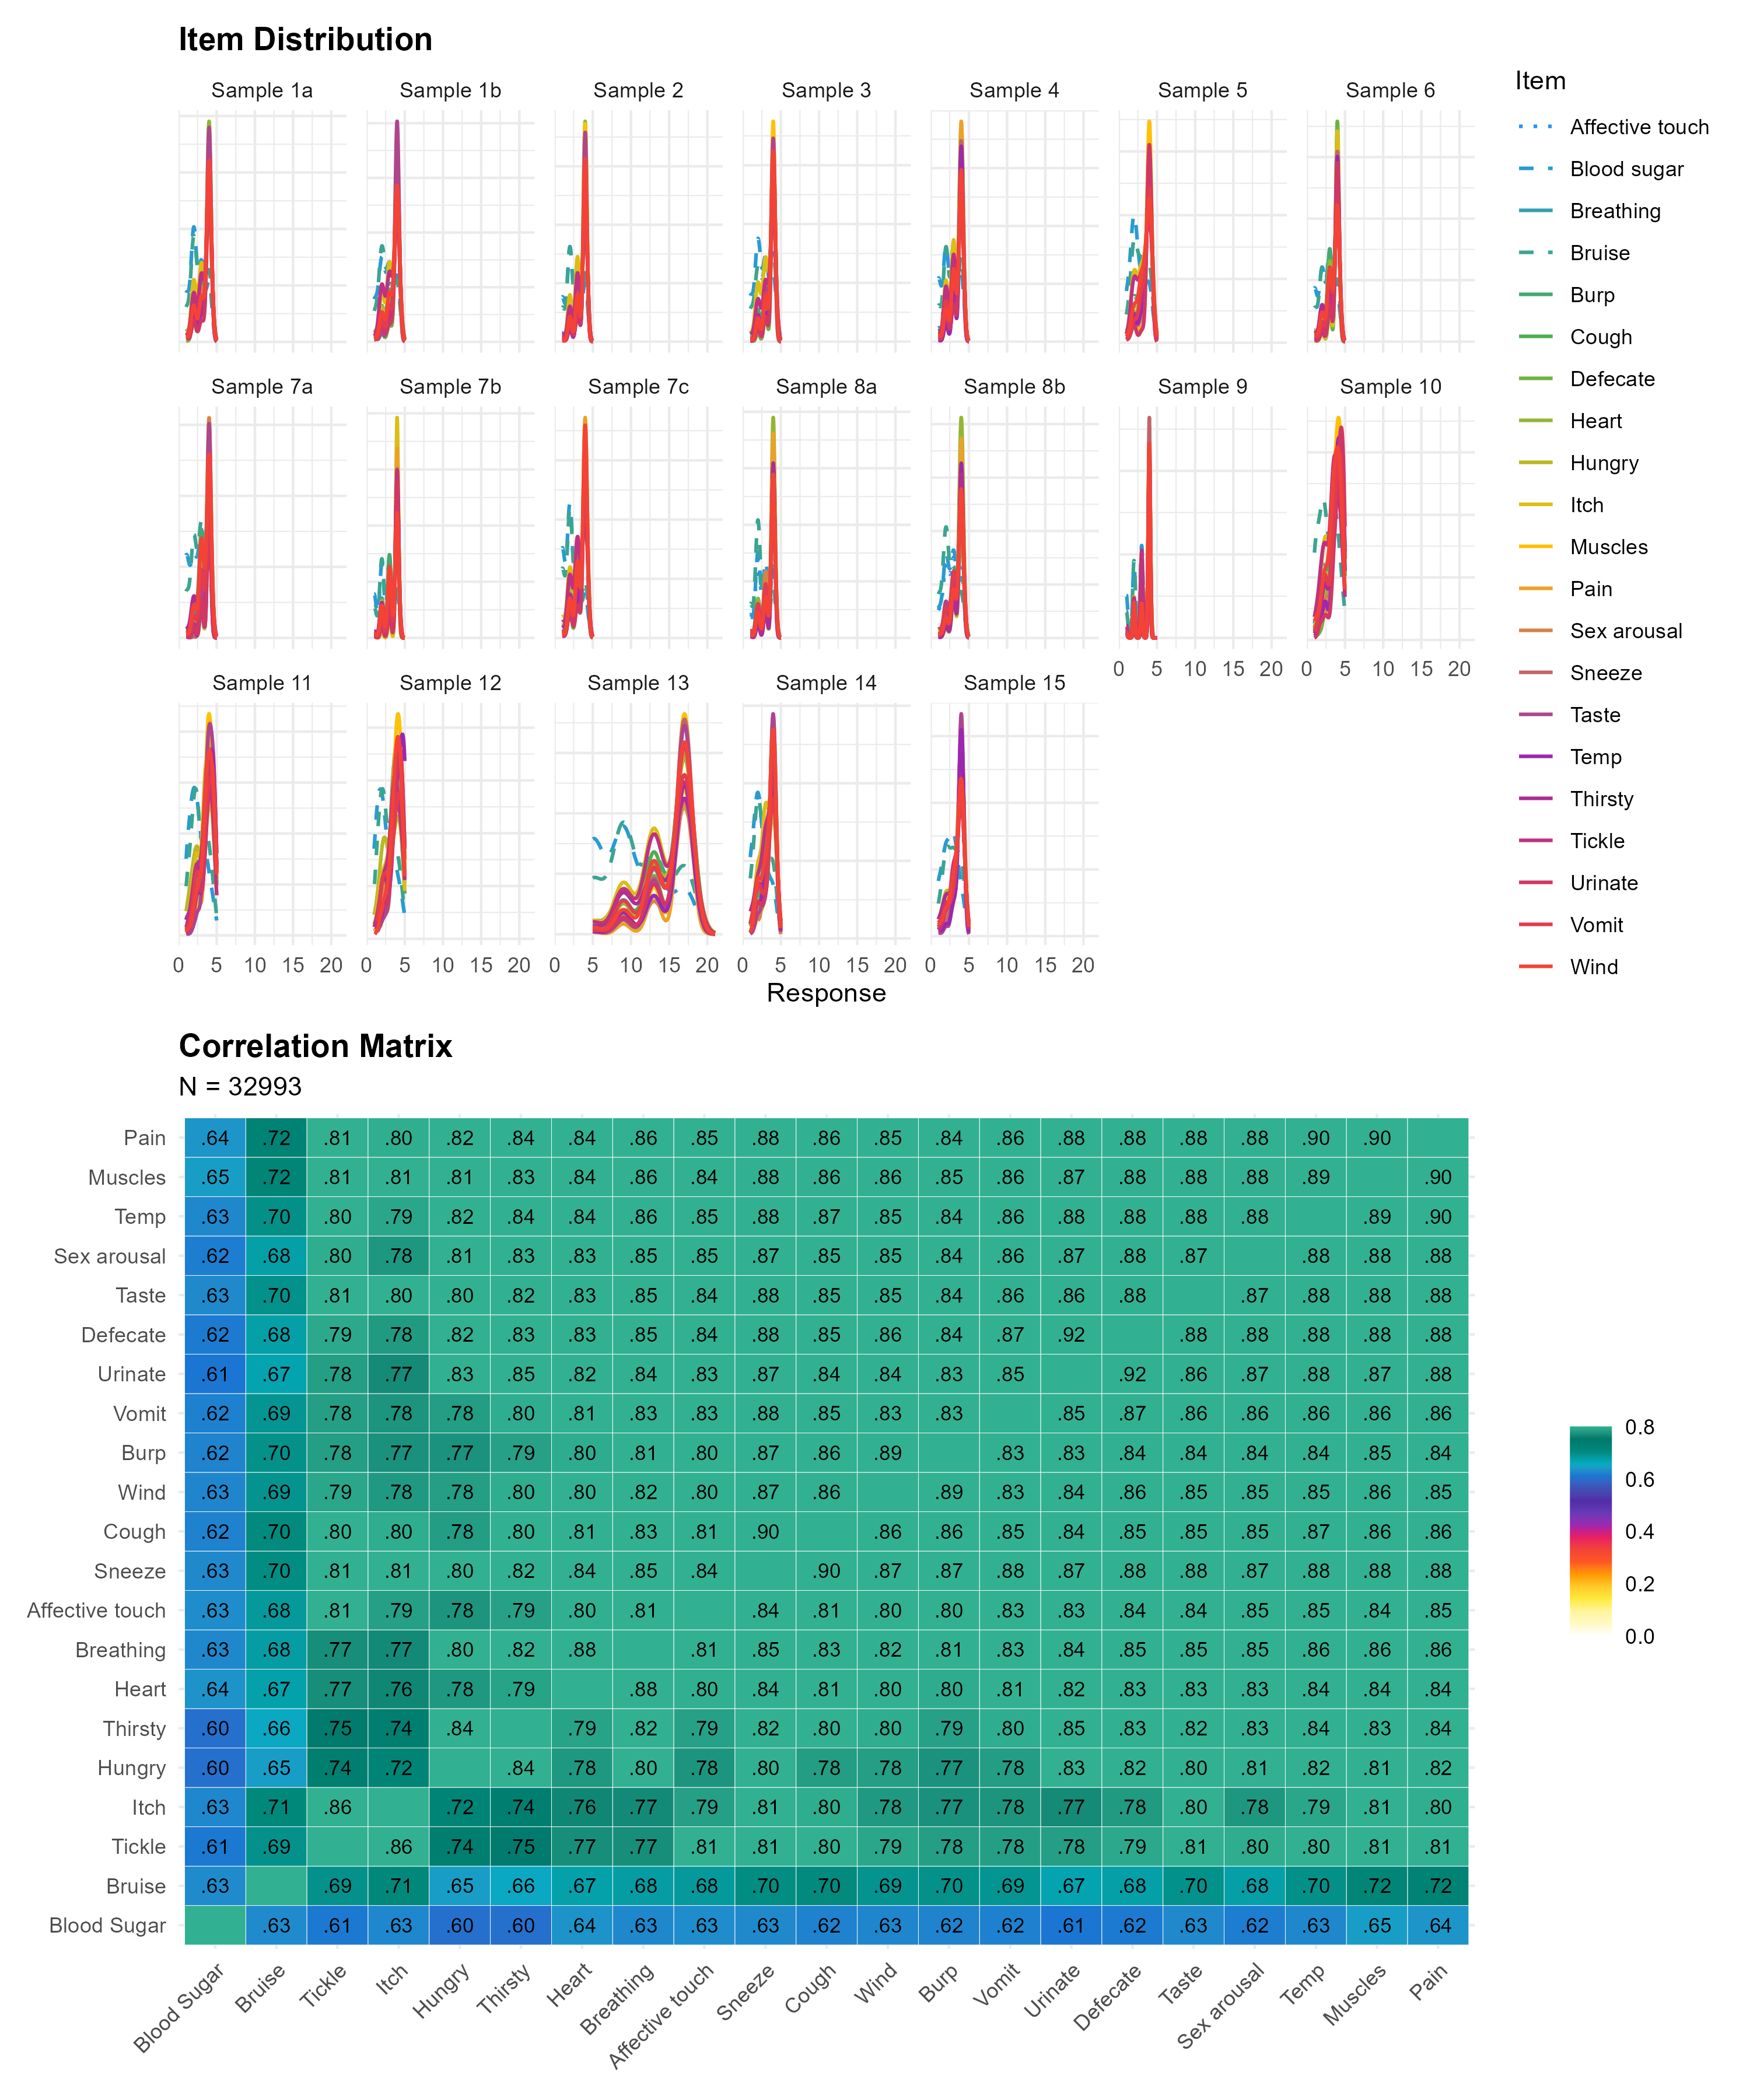
\includegraphics[width=1\linewidth,height=\textheight,keepaspectratio]{../../analysis/figures/Figure1.png}

\end{figure*}

UVA flagged two strongly redundant variables, ``itch'' and ``tickle'' -
suggesting to remove the latter. Several more pairs of items were
flagged as moderately redundant (``wind'' and ``burp''; ``urinate'' and
``defecate'') and mildly redundant (``sneeze'' and ``cough''; ``heart''
and ``breathing''; ``hungry'' and ``thirsty''). These patterns
consistently appeared in most samples when considered individually. We
removed ``tickle'' from further analysis due to its high redundancy (and
because it is absent from some datasets due to translation issues).

The HCA highlighted pairs and triplets of items consistently grouped
together across samples, such as ``wind'' and ``burp'', ``sneeze'' and
``cough'', ``itch'' and ``bruise'', ``urinate'' and ``defecate'', and
``pain'', ``muscles'', and ``temperature''. This pattern was largely
replicated by the EGA, with the additional presence of a unique cluster
comprising ``Sex arousal'', ``Affective touch'', ``Temperature'',
``Pain'', ``Muscles'', and ``Taste''. EFA suggested the optimal number
of factors to be 3, yielding one dimension with expulsion-related items
(``burp'', ``wind'', ``cough'', ``sneeze'', and ``vomit''), a second
dimension with visceroceptive items (``heart'', ``breathing'',
``hungry'', ``thirsty'', ``urinate'', and ``defecate''), and a third
dimension with skin-related items (``bruise'' and ``blood sugar'').

Importantly, this initial structure analysis run highlighted some
problematic items: ``taste'' typically displayed a lone or unstable
pattern of associations, ``affective touch'' exhibited cross-loadings
and instability, ``vomit'' was less strongly associated with other
items, and ``itch'' did not form a consistent cluster. Finally,
``temperature'' and ``sexual arousal'' showed redundant patterns of
associations but were less reliable. These 6 items were thus removed,
and a second run of structure analysis was performed on the remaining 14
items.

\begin{figure*}[!htbp]

{\caption{{TODO.}{\label{fig-structure}}}}

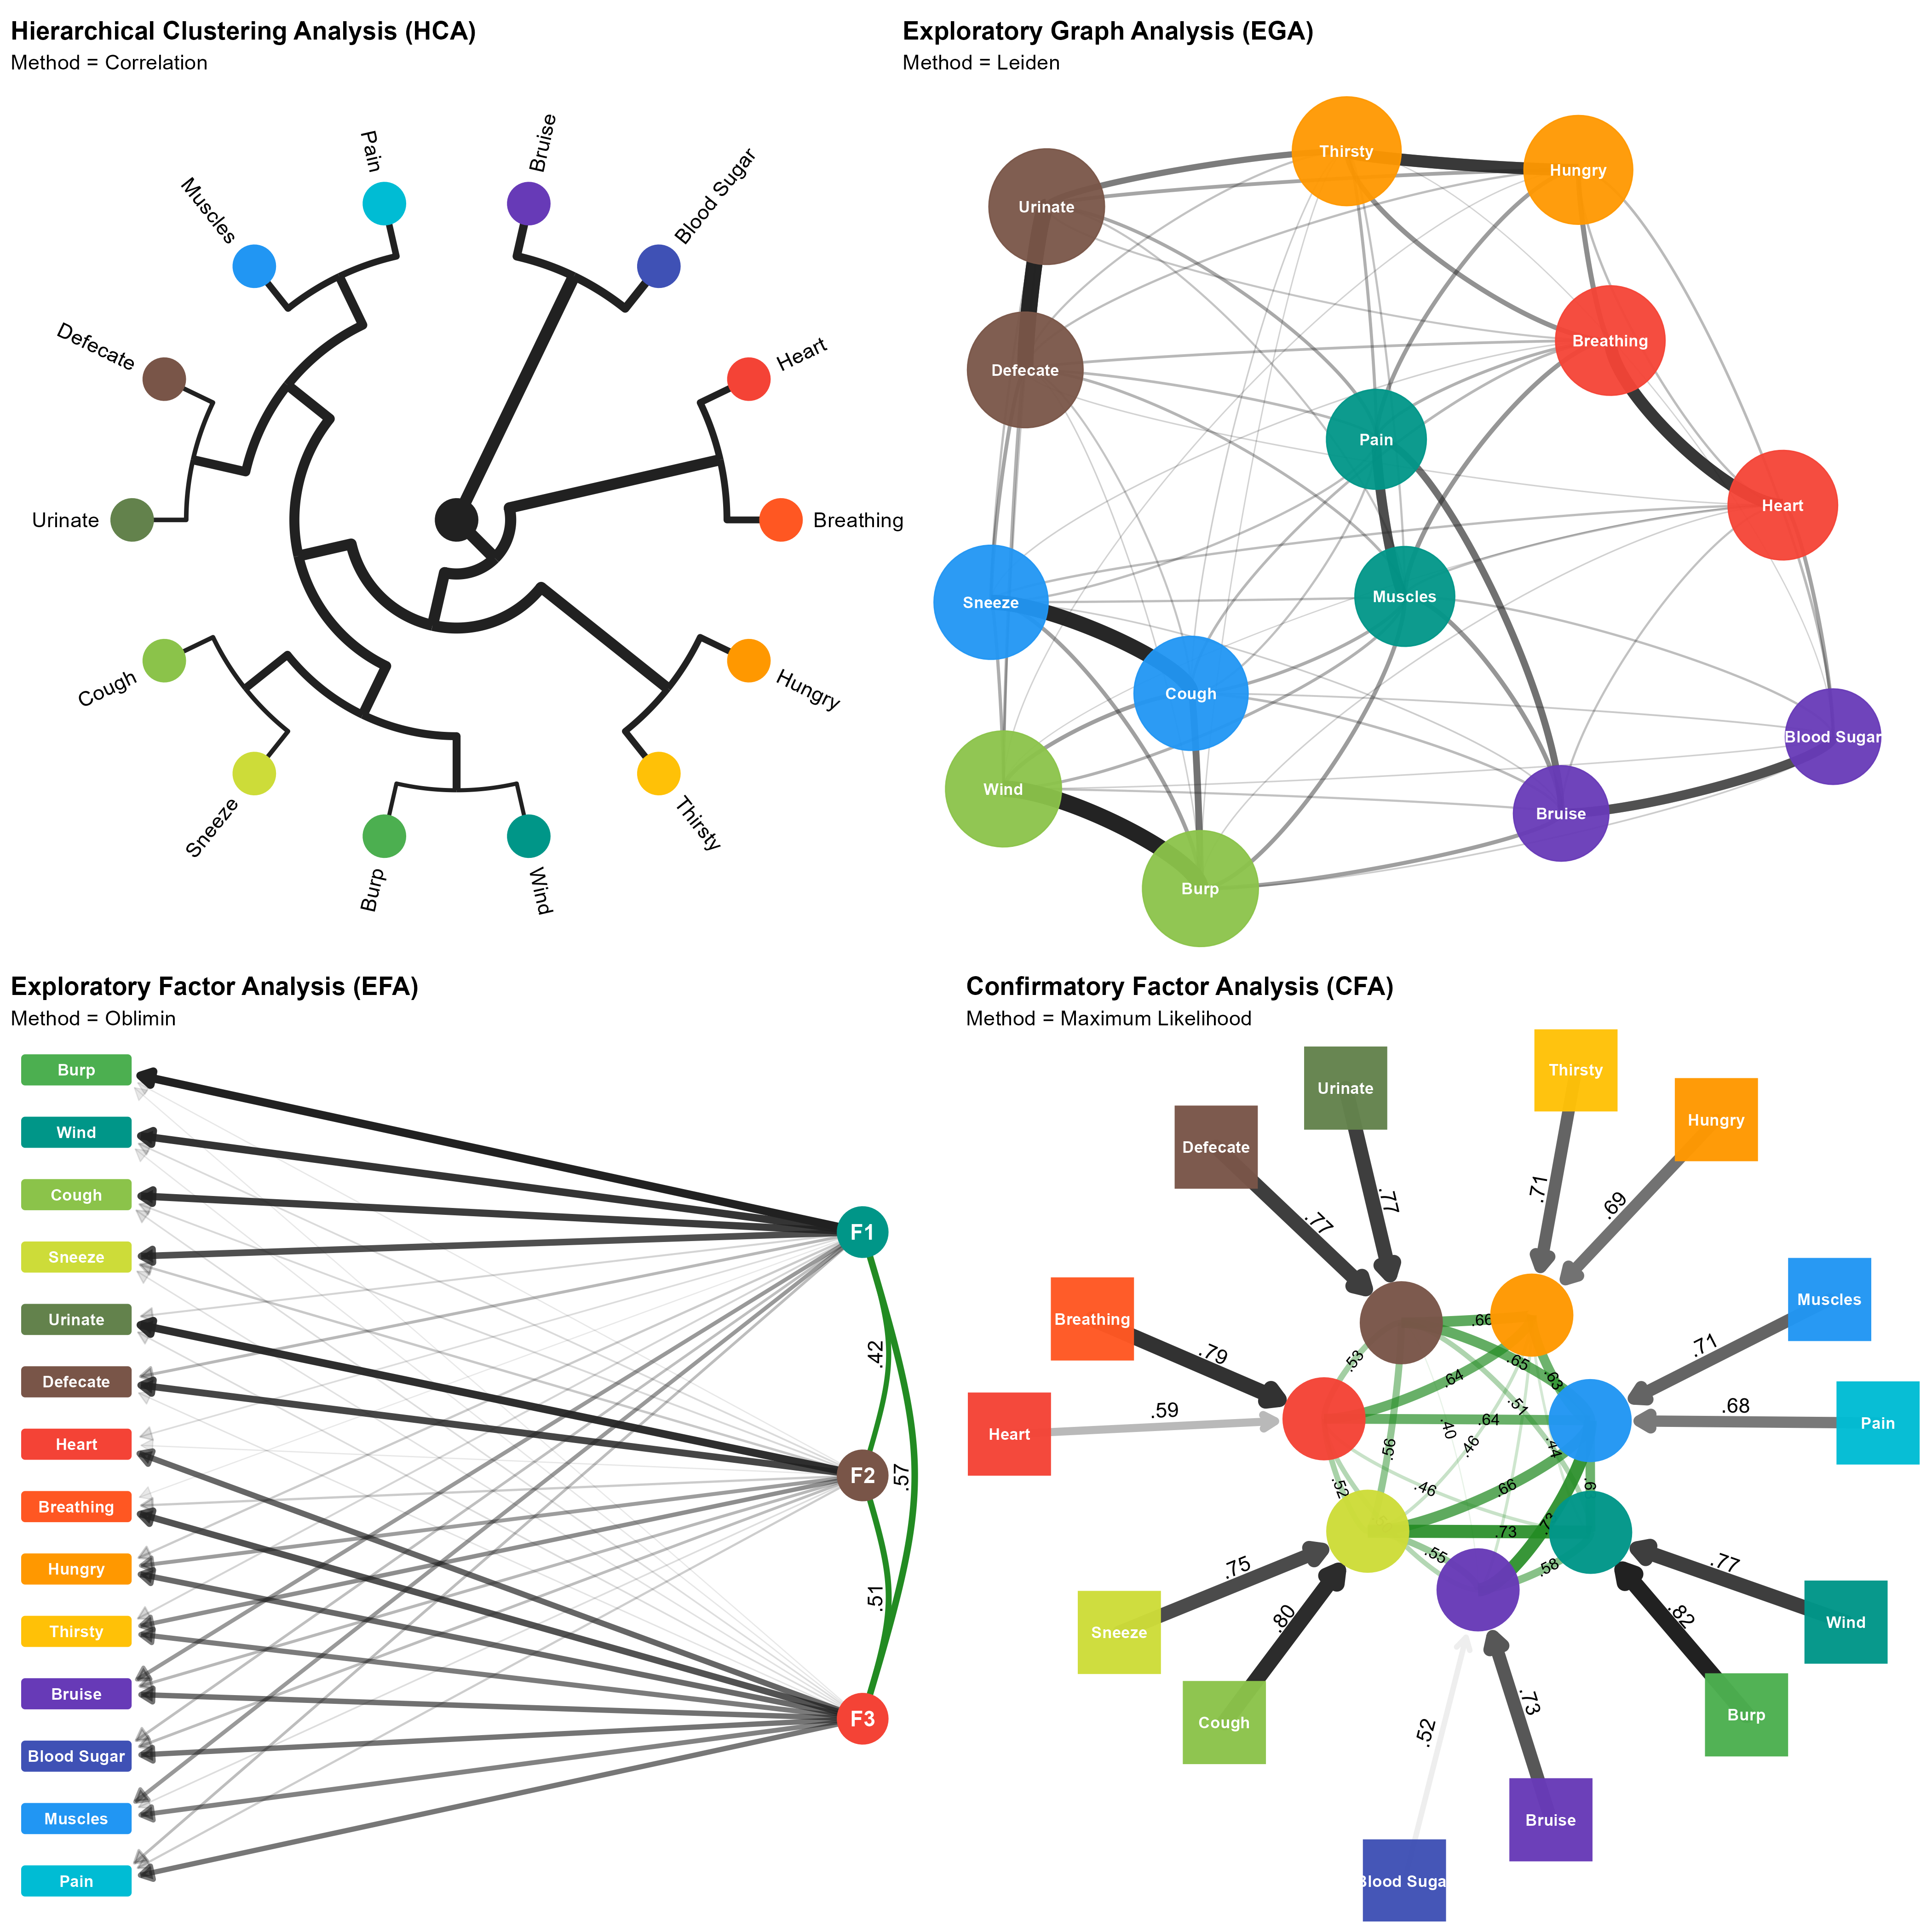
\includegraphics[width=1\linewidth,height=\textheight,keepaspectratio]{../../analysis/figures/Figure2.png}

\end{figure*}

HCA and EGA yielded highly consistent results, emphasizing pairs of
items, namely Hungry-Thirsty, Bruise-Blood sugar, Urinate-Defecate,
Muscles-Pain, Breathing-Heart, Cough-Sneeze, Wind-Burp. HCA also
significantly grouped the Urinate-Defecate and Muscles-Pain pairs, as
well as expulsion items (Wind-Burp and Cough-Sneeze). EFA suggested once
again 3 factors as the optimal solution, with the first factor including
expulsion-related items (``burp'', ``wind'', ``cough'', ``sneeze''), the
second factor being related to the Urinate-Defecate pair, and the third
factor comprising the remaining items.

We then fitted and compared using CFA various candidate structures
emerging from the previous analyses, including a 1-factor model (the
G-model), a 3-factor model (EFA), a 3+1 model (EFA + general factor), a
5-factor model (HCA), a 5+1 model (HCA + general factor), a 7-factor
model (EGA), and a 7+1 model (EGA + general factor). The EGA model with
7 factors of item pairs provided the best fit with the lowest RMSEA
(0.035), lowest \(\chi^2\) (2306.30), highest CFI (0.984). It was
followed by the EGA + general factor model (RMSEA = 0.054, \(\chi^2\) =
6842.38, CFI = 0.952), and the HCA model with 5 factors (RMSEA = 0.078,
\(\chi^2\) = 13296.33, CFI = 0.907). The other models performed poorly,
with RMSEA \textgreater{} 0.08 and CFI \textless{} 0.90. The
unique-factor model yielded the lowest BIC (which takes into account the
number of factors), followed by the EGA model. All the other models
displayed significantly (BIC-based Bayes Factor \textless{} 1/100) lower
evidence compared to the EGA model.

This result was relatively consistent across unique datasets with the
EGA model providing the best fit. In all samples where CFA converged, it
showed excellent performance with low RMSEA (≈ 0.025--0.046), high CFI
(≥ 0.97), and substantially lower \(\chi^2\) compared to alternative
models. Adding a general factor systematically worsened fit, while
hierarchical clustering and EFA-based models showed poorer performance
(RMSEA \textgreater{} 0.06, CFI \textless{} 0.93). Although BIC values
occasionally favored alternative specifications, Bayes factor
comparisons overwhelmingly supported the EGA solution, confirming its
robustness across datasets.

\subsection{Discussion}\label{discussion}

The first study aimed to provide the most systematic test of the IAS
structure to date. Previous work has produced conflicting models,
ranging from a single general factor (\citeproc{ref-brand2023}{Brand et
al., 2023}), to bifactor solutions (\citeproc{ref-campos2021}{Campos et
al., 2021}; \citeproc{ref-lin2023}{Lin et al., 2023}), and two-factor
models (\citeproc{ref-koike2023}{Koike \& Nomura, 2023};
\citeproc{ref-murphy2019}{Murphy et al., 2019}). Alongside these
structural discrepancies, several studies have questioned the quality of
specific items. Murphy et al. (\citeproc{ref-murphy2019}{2019})
distinguished between items tapping direct interoceptive signals (e.g.,
heartbeat) and others reflecting phenomena less accessible to
interoception (e.g., bruising). Additionally, Lin et al.
(\citeproc{ref-lin2023}{2023}) identified locally dependent pairs and
low-discrimination items with Network-based methods, while Campos et al.
(\citeproc{ref-campos2021}{2021}) found that ``tickle'' did not load on
the general factor. To address these open questions, we reanalyzed
multiple open-access datasets using a mega-analytic framework,
contrasting traditional factor-analytic approaches with network-based
methods.

Overall, the findings converge on a robust yet novel picture. Initial
analysis revealed issues in 7 items (e.g., instability, redudancy, low
associations, less reliable) which led to the formation of a 14-item
IAS. Exploratory and confirmatory analyses indicated that the IAS is
best characterized by seven pairs of closely related items, consistently
identified by EGA and supported by HCA. These pairs (e.g.,
hunger--thirst, urinate--defecate, cough--sneeze) were highly replicable
across independent samples and yielded superior fit indices in CFA
compared to other solutions. Although the one-factor model occasionally
achieved lower BIC, Bayes factor comparisons overwhelmingly supported
the EGA structure, underlining its empirical robustness.

This pattern has several important implications. First, it suggests that
the IAS does not capture a broad latent construct of interoceptive
accuracy as originally intended, but rather reflects a set of tightly
coupled item clusters tied to specific bodily sensations. In other
words, the IAS may function more as a checklist of bodily signal
detection items than as a scale measuring a coherent higher-order
dimension. This stands in contrast to the original two-factor proposal
(\citeproc{ref-murphy2019}{Murphy et al., 2019}), where the factors were
highly correlated and collapsed into a unidimensional score, and helps
explain why subsequent studies diverged in their conclusions: the
psychometric structure of the IAS appears to be driven more by local
dependencies than by robust latent factors. Second, the presence of
redundant or unstable items (e.g., tickle, taste, affective touch),
already highlighted in prior validation studies
(\citeproc{ref-campos2021}{Campos et al., 2021};
\citeproc{ref-lin2023}{Lin et al., 2023}), undermines the
interpretability of the scale, as their contributions appear
inconsistent or overlapping. Together, these findings help explain why
previous research has struggled to converge on a stable factor
structure: the IAS lacks the psychometric properties required for strong
latent modeling and may overstate its dimensionality by conflating
redundancy with structure.

At the same time, the results do not render the IAS unusable. The
consistent emergence of item pairs highlights intuitive bodily domains
(e.g., visceral, expulsion, musculoskeletal) that align with everyday
interoceptive experiences, supporting its ecological validity. However,
the limited breadth of these pairings, the redundancy across items, and
the reliance on a narrow 5-point scale all restrict the scale's ability
to differentiate between individuals and to capture the multidimensional
nature of interoception (\citeproc{ref-desmedt2022measures}{Desmedt et
al., 2022}). These findings therefore call for refinement, either
through targeted revisions of the IAS (e.g., removing redundant items,
addition of context-specific items, adopting analogue response formats)
or through the development of a new questionnaire that better balances
theoretical coherence with empirical validity.

In sum, Study 1 demonstrates that the IAS structure is best described by
clusters of tightly coupled item pairs reflecting local dependencies,
rather than by a broad latent dimension. While this solution is
replicable and statistically robust, it highlights the conceptual and
psychometric limitations of the IAS in its current form. These insights
help contextualize the mixed findings on the scale's validity and
provide a crucial foundation for Study 2, where we do the dispositional
correlates of the IAS to further evaluate its construct validity and
situate it within the broader network of interoceptive and psychological
traits.

\section{Study 2}\label{study-2}

\subsection{Study 2}\label{study-2-1}

Building on the structural findings from Study 1, the second study turns
to the validity of the IAS by examining its dispositional correlates.
Although the IAS has been widely used, evidence regarding its
associations with personality traits, affective dispositions, and
related psychological constructs remains scattered and inconsiste
(\citeproc{ref-brand2023}{Brand et al., 2023};
\citeproc{ref-lin2023}{Lin et al., 2023};
\citeproc{ref-murphy2019}{Murphy et al., 2019};
\citeproc{ref-todd2022}{Todd et al., 2022}). Study 2 therefore had two
primary goals. First, to provide a robust overview of the dispositional
correlates of the IAS by leveraging the large number of available
datasets. Second, to evaluate the practical benefits of using the
refined 14-item version of the scale identified in Study 1, compared to
the original 21-item unidimensional version, in order to assess whether
structural improvements translate into clearer and more reliable
external associations.

\subsection{Methods}\label{methods-1}

\subsubsection{Materials}\label{materials}

We selected measures that appeared in multiple datasets from Study 1
and/or were relevant given the scope of the study, merging scores of
regular and abridged versions for conciseness where applicable. The
measures include constructs related to interoception, mood, personality,
psychopathology, and beliefs and misbeliefs.

\paragraph{Interoception Related.}\label{interoception-related}

The Multidimensional Assessment of Interoceptive Awareness Version-2
(MAIA-2, \citeproc{ref-mehling2018multidimensional}{Mehling et al.,
2018}) is a 37-item questionnaire assessing eight dimensions of
interoception: Noticing, Not-Distracting, Not-Worrying, Attention
Regulation, Emotional Awareness, Self-Regulation, Body Listening, and
Trust. Responses are rated on a 6-point Likert scale (e.g., ``I notice
when I am uncomfortable in my body'').

The Body Perception Questionnaire Short Form (BPQ-SF,
\citeproc{ref-cabrera2018assessing}{Cabrera et al., 2018}) contains 46
items measuring body awareness and autonomic reactivity on a 5-point
Likert scale (e.g., ``My heart often beats irregularly''). The
very-short form (BPQ-VSF) contains 12 items from the body awareness
subscale. For this study, scores from both versions were combined.

The Interoceptive Confusion Questionnaire (ICQ,
\citeproc{ref-brewer2016alexithymia}{Brewer et al., 2016}) consists of
20 items rated on a 5-point Likert scale (e.g., ``I cannot tell when my
muscles are sore or tight'') assessing difficulties in interpreting
non-affective physiological states, such as pain or hunger.

The Toronto Alexithymia Scale (TAS-20,
\citeproc{ref-bagby1994twenty}{Bagby et al., 1994}) contains 20 items
rated on a 5-point forced-choice scale (e.g., ``I have feelings I can't
quite identify''), divided into three dimensions: difficulty identifying
feelings, difficulty describing feelings, and externally oriented
thinking.

The Bermond--Vorst Alexithymia Questionnaire (BVAQ,
\citeproc{ref-vorst2001validity}{Vorst \& Bermond, 2001}) consists of 40
items across five subscales: fantasising, identifying, analysing,
verbalising, and emotionalising. Items are rated on a 5-point Likert
scale. The BVAQ also provides two higher-order factors, namely affective
and cognitive (e.g., ``I like to tell others how I feel'').

\paragraph{Mood and Anxiety Related.}\label{mood-and-anxiety-related}

The Beck Depression Inventory-II (BDI-II,
\citeproc{ref-beck1996beck}{Beck et al., 1996}) is a 21-item measure of
depressive symptom severity, including psychological (e.g., guilt) and
physiological (e.g., loss of energy) components. Items are rated on a
4-point scale (e.g., ``I feel sad much of the time'').

The Patient Health Questionnaire-4 (PHQ-4,
\citeproc{ref-kroenke2009ultra}{Kroenke et al., 2009}) is a 4-item
screening tool for depression and anxiety, rated on a 4-point Likert
scale (e.g., ``Little interest or pleasure in doing things''; ``Not
being able to stop or control worrying''). The PHQ-2 (PHQ-2,
\citeproc{ref-kroenke2003patient}{Kroenke et al., 2003}) and General
Anxiety Disorder-2 (GAD-2, \citeproc{ref-kroenke2007anxiety}{Kroenke et
al., 2007}) scores were combined with the PHQ-4 scores.

The Patient Health Questionnaire-9 (PHQ-9,
\citeproc{ref-kroenke2001phq}{Kroenke et al., 2001}) includes 9 items
assessing depressive symptoms on a 4-point Likert scale (e.g., ``Feeling
tired or having little energy?'').

The Patient Health Questionnaire-15 (PHQ-15,
\citeproc{ref-kroenke2002phq}{Kroenke et al., 2002}) assesses somatic
symptom distress with 15 items rated on a 3-point scale (e.g., ``Over
the last week, how often have you been bothered by back pain?'').

The Short Mood and Feelings Questionnaire (SMFQ,
\citeproc{ref-angold1995development}{Angold et al., 1995}) is a 13-item
measure of recent depressive symptoms in children aged 6--17, rated on a
3-point scale (e.g., ``I felt miserable or unhappy'').

The State--Trait Anxiety Inventory Trait Version (STAI-T,
\citeproc{ref-spielberger1970manual}{Spielberger, 1970}) is a 20-item
trait anxiety questionnaire rated on a 4-point Likert scale (e.g., ``I
worry too much about something that really doesn't matter''). Scores
from the shorter version of the STAIT-5
(\citeproc{ref-zsido2020development}{Zsido et al., 2020}) were combined
with the STAI-T.

The Generalized Anxiety Disorder Scale (GAD-7,
\citeproc{ref-spitzer2006brief}{Spitzer et al., 2006}) is a 7-item
measure of generalized anxiety symptoms rated on a 4-point Likert scale
(e.g., ``Not being able to stop or control worrying'').

\paragraph{Personality.}\label{personality}

The NEO Five-Factor Inventory, neuroticism subscale (NEO-FFI,
\citeproc{ref-costa1992neo}{Costa \& McCrae, 1992}) is a 12-item measure
of neuroticism, assessing the general tendency to experience negative
emotions such as fear, sadness, or disgust. Items are rated on a 5-point
Likert scale (e.g., ``I often feel inferior to others'').

The Mini International Personality Item Pool (MINI-IPIP6,
\citeproc{ref-sibley2011mini}{Sibley et al., 2011}) includes 24 items
measuring six broad traits: Agreeableness, Conscientiousness,
Neuroticism, Openness, Extraversion, and Honesty-Humility. Items were
scored on visual analogue scales in our samples (originally 7-point
Likert scales; e.g., ``Have a vivid imagination'').

The Big Five Inventory Short Form (BFI-S,
\citeproc{ref-rammstedt2007measuring}{Rammstedt \& John, 2007}) is a
10-item measure of the Big Five traits, rated on a 7-point Likert scale
(e.g., ``I see myself as someone who \ldots{} is considerate and kind to
almost everyone'').

\paragraph{Psychopathology.}\label{psychopathology}

The Personality Inventory for DSM-5 Short Form (PID-5-SF,
\citeproc{ref-thimm2016personality}{Thimm et al., 2016}) consists of 25
items rated on a 4-point Likert scale, measuring five domains:
disinhibition, antagonism, detachment, negative affect, and psychoticism
(e.g., ``Plenty of people are out to get me'').

The Schizotypal Personality Questionnaire -- Brief Revised (SPQ-BR,
\citeproc{ref-davidson2016schizotypal}{Davidson et al., 2016}) contains
32 items rated on a 5-point Likert scale, assessing four primary
dimensions: cognitive-perceptual, interpersonal, disorganized, and
social anxiety. These are subdivided into nine secondary factors,
including constricted affect, eccentricity, magical thinking, lack of
close friends, odd speech, referential thinking, social anxiety,
suspiciousness, and unusual perceptions (e.g., ``Plenty of people are
out to get me'').

The McLean Screening Instrument for Borderline Personality Disorder
(MSI-BPD, \citeproc{ref-zanarini2003zanarini}{Zanarini, 2003}) is a
10-item dichotomous screening measure for borderline personality
disorder (present/absent; e.g., ``Have any of your closest relationships
been troubled by a lot of arguments or repeated breakups?'').

The Autism Spectrum Quotient Short Form (ASQ-S,
\citeproc{ref-hoekstra2011construction}{Hoekstra et al., 2011}) is a
28-item measure of five autistic traits: social skills, adherence to
routines, cognitive flexibility, imagination, and patterns/numbers.
Items are rated on a 4-point Likert scale (e.g., ``I find it difficult
to work out people's intentions'').

\paragraph{Beliefs and Misbeliefs.}\label{beliefs-and-misbeliefs}

The Generic Conspiracist Beliefs Scale (GCBS,
\citeproc{ref-brotherton2013measuring}{Brotherton et al., 2013}) is a
15-item measure assessing five dimensions of conspiracy beliefs:
government malfeasance, extraterrestrial cover-up, malevolent global
conspiracies, personal wellbeing, and control of information. Items are
scored on a 5-point Likert scale (e.g., ``Secret organizations
communicate with extraterrestrials, but keep this fact from the
public'').

The Primal World Beliefs Inventory (PI-99,
\citeproc{ref-clifton2019primal}{Clifton et al., 2019}) is a 99-item
measure assessing 26 high-order beliefs about the world. Items are
scored on a 5-point Likert scale (e.g., ``Nearly everything in the world
is beautiful'') The PI-18 (\citeproc{ref-clifton2021brief}{Clifton \&
Yaden, 2021}) is a short form of the orginal questionnaire assessing the
4 main world beliefs: the world is Good (vs.~Bad) and its three
dimensions: Safe (vs.~Dangerous), Enticing (vs.~Dull), and Alive
(vs.~Mechanistic). Scores from the PI-18 scores were combined with the
PI-99.

The Lie Scale (LIE, \citeproc{ref-makowski2023structure}{Makowski et
al., 2023}) is a 16-item measure of lying tendencies across four
components: Ability, Frequency, Negativity, and Contextuality. Items are
scored on visual analogue scales (e.g., ``I am a good liar'').

\subsubsection{Data Analysis}\label{data-analysis-1}

All variables from the 16 open-access datasets will be extracted and
standardized (z-scored). For continuous predictors, we will first ensure
consistent ranges across datasets; when necessary, ranges will be
rescaled to achieve comparability. In cases where scales of different
lengths measure the same construct, scores will be harmonized: when
possible, means will be computed from overlapping items, while in other
cases total scores will be normalized by the number of items. We will
collapse redundant subscales (e.g., PHQ-2 and GAD-2 within PHQ-4) into
unified composite scores. Similarly, short forms of trait anxiety (e.g.,
STAI-5-trait) will be collapsed with their longer counterpart (STAI-T),
with scores computed as the mean to ensure comparable ranges. Shorter
formats of the PI (PI-18) will be combined with scores of its longer
version (PI-99). Missing data will be handled via listwise deletion on a
per-model basis prior to fitting.

Associations will be estimated using multilevel regression models
implemented in the glmmTMB package (\citeproc{ref-glmTMB}{McGillycuddy
et al., 2025}). Each predictor will be entered separately, with the
seven IAS item pairs identified in Study 1 (``Hungry--Thirsty'',
``Muscles--Pain'', ``Wind--Burp'', ``Urinate--Defecate'',
``Breathing--Heart'', ``Bruise--Blood'', ``Cough--Sneeze'') and the
original IAS scale serving as outcomes. Models will include random
intercepts and slopes by sample to account for between-study
heterogeneity; when models fail to converge, a reduced structure with
random intercepts only will be used. This approach will treat datasets
as clusters, thereby providing pooled estimates of the associations
while accounting for both within- and between-sample variability, akin
to a meta-analytic framework.

From each fitted model, we will extract standardized regression
coefficients (β), 95\% confidence intervals, p-values, convergence
status, and effective sample size. Participants identifying as ``Other''
will be excluded from analyses due to limited representation.

\subsection{Results}\label{results-1}

Age was positively associated across Ias correlates (mean r = .12), with
all correlations significant. Gender showed near-zero effects (mean r =
−.01), with 63\% reaching significance.

Several MAIA subscales showed consistent positive associations with the
IAS: Noticing, Attention Regulation, Trusting, Emotional Awareness,
Listening, and Self-Regulation (βs ≈ .18--.26). These effects were
generally strongest for the full IAS, but often replicated with
Hungry/Thirsty or Bruise/Blood pairings. By contrast, Autonomic
Reactivity (BPQ; β = −.17) was reliably negative across most pairings,
while Body Awareness (BPQ; β = .12) was weak and only reliable for
Hungry/Thirsty and Bruise/Blood. Alexithymia measures were consistently
negative, with robust effects across both the full IAS and pairings,
except for the Affective dimension of the BVAQ which showed only a
positive association with the Bruise/Blood sugar pairing (β = .04).

Depression (BDI; β = −.20) and anxiety (STAI-T; β = −.19) were
consistently negative across the IAS and most pairings, with
Hungry/Thirsty again emerging as a particularly sensitive correlate.
Broader symptom indices (PHQ-15, PHQ-4, GAD-7) showed weaker but often
reliable effects, although some were restricted to certain pairings
(e.g., PHQ-15 with Hungry/Thirsty, Bruise/Blood). By contrast, PHQ-9 and
MFQ averaged negatively but were largely nonsignificant, even with the
full scale. Autistic traits were generally negative, especially
Imagination (β = −.18), which showed broad consistency across pairings
except Cough/Sneeze.

Within the Big Five, Openness (β = .14), Agreeableness (β = .05), and
Conscientiousness (β = .03) showed small but consistent positive
associations, most reliably captured by the full IAS but also evident in
pairings. Honesty--Humility was uniquely negative, with significant
associations for both the full scale and Hungry/Thirsty. Worldview
measures were generally null, though belief in a comprehensible world (β
= .11) and an ``alive'' world (β = .09) showed small but consistent
positive associations, mainly with the full IAS and Hungry/Thirsty.

Overall, the full IAS yielded the largest number of significant
associations (25), but the Hungry/Thirsty (16) and Bruise/Blood sugar
(11) pairings frequently showed equally strong or stronger effects.
These item-level pairings often captured variance that the full scale
did not, particularly for interoceptive and mood measures. In contrast,
other pairings (e.g., Cough/Sneeze, Wind/Burp, Urinate/Defecate)
contributed little unique variance. Together, these results suggest that
while the full IAS captures broad dispositional tendencies, select
pairings may provide more fine-grained sensitivity to specific domains,
particularly interoception and affect.

{[}\textbf{NOTE} justify the choice of those specific primals ? higehr
correlations with the IAS?{]}

\subsection{Discussion}\label{discussion-1}

The second study set out to provide a comprehensive overview of the
dispositional correlates of the IAS by pooling data across multiple
datasets, while also testing whether the refined 14-item version
identified in Study 1 confers practical advantages over the original
21-item scale.

Consistent with prior research, the IAS showed strong positive
associations with other interoceptive self-report measures, particularly
the MAIA, with the exception of the Not Distracting and Not Worrying
facets (\citeproc{ref-brand2023}{Brand et al., 2023}). This pattern
replicates earlier findings while contradicting
(\citeproc{ref-todd2022}{Todd et al., 2022}), who reported only a
near-zero correlation with Not Worrying. Similarly, while previous
evidence on the BPQ was mixed, our results indicate more robust
associations with the Autonomic Reactivity dimension compared to body
awareness (\citeproc{ref-brand2023}{Brand et al., 2023};
\citeproc{ref-campos2021}{Campos et al., 2021};
\citeproc{ref-todd2022}{Todd et al., 2022}). This pattern diverges from
earlier findings that consistently reported significant positive
associations with Body Awareness (\citeproc{ref-brand2023}{Brand et al.,
2023}; \citeproc{ref-campos2021}{Campos et al., 2021};
\citeproc{ref-gaggero2021}{Gaggero et al., 2021}), while at the same
time complementing reports of significant negative correlations with
Autonomic Reactivity (\citeproc{ref-gaggero2021}{Gaggero et al., 2021}).
The replication of negative associations with interoceptive confusion
(\citeproc{ref-brand2023}{Brand et al., 2023};
\citeproc{ref-gaggero2021}{Gaggero et al., 2021};
\citeproc{ref-murphy2019}{Murphy et al., 2019}) further supports the
convergent and discriminant validity of the IAS.

Robust negative correlations were observed between the IAS and
alexithymia, in line with prior studies (\citeproc{ref-brand2023}{Brand
et al., 2023}; \citeproc{ref-campos2021}{Campos et al., 2021};
\citeproc{ref-koike2023}{Koike \& Nomura, 2023};
\citeproc{ref-lin2023}{Lin et al., 2023};
\citeproc{ref-murphy2019}{Murphy et al., 2019}). Similarly, negative
associations with depression and anxiety, as measured by the BDI and
STAI-T, reinforce the clinical relevance of interoceptive accuracy
(\citeproc{ref-brand2023}{Brand et al., 2023};
\citeproc{ref-lin2023}{Lin et al., 2023}). Somatic symptoms were also
negatively related to the IAS, although effect sizes were small, echoing
earlier findings (\citeproc{ref-brand2023}{Brand et al., 2023};
\citeproc{ref-koike2023}{Koike \& Nomura, 2023};
\citeproc{ref-lin2023}{Lin et al., 2023}). At the same time, more recent
studies have reported null or inconsistent associations between
interoceptive sensitivity and mental-health symptomatology, suggesting
that such links may not generalize across all interoceptive domains and
could be contingent on measurement approaches or sample characteristics
{[}\textbf{REF PRE\_PRINT?}{]}.

Clear negative associations also emerged with autism-related traits such
as imagination, low attentional switching, and reduced social skills.
These findings resonate with DuBois et al.
(\citeproc{ref-dubois2016}{2016}) review reporting interoceptive
abnormalities in autism. Nonetheless, our findings are limited to a
single dataset employing the ASQ, which constrains the generalisability
of conclusions regarding the relationship between interoception and
autistic traits.

The associations between interoception and personality traits were more
nuanced. Whereas prior work suggested a negative link with neuroticism
(\citeproc{ref-brand2023}{Brand et al., 2023}), we found this
relationship to be inconsistent and even slightly positive, though near
zero. By contrast, openness and agreeableness were consistently
positively associated with the IAS, albeit with small effect sizes.
These findings are consistent with emerging evidence linking openness to
interoception as measured by the MAIA-2
(\citeproc{ref-simkute2025interoception}{Simkute et al., 2025}), and
complement reports of associations between interoceptive sensitivity
(i.e., the accuracy of reported heartbeat counts relative to actual
heartbeats) and extraversion
(\citeproc{ref-haustein2024interoception}{Haustein et al., 2024}).
Personality effects more broadly were modest in size, and as such,
warrant replication before firm conclusions can be drawn. In contrast,
maladaptive personality dimensions and schizotypal traits showed only
weak and inconsistent associations with the IAS, indicating that
interoceptive accuracy may not play a central role in these domains.

Beyond established correlates, exploratory analyses revealed weak but
positive associations between the IAS and primal world beliefs,
specifically perceiving the world as alive and understandable. The
inclusion of primal world beliefs was exploratory, motivated by their
potential theoretical link to embodied cognition and meaning-making
processes. Although effect sizes were small, the emergence of consistent
associations with perceiving the world as alive and understandable
suggests an intriguing avenue for future work at the intersection of
interoception and worldview formation.

A central aim of Study 2 was to assess whether the refined 14-item IAS
identified in Study 1 provides practical benefits over the original
21-item scale. While the full version most often emerged as the
strongest correlate, the refined 14-item IAS performed largely
comparably across dispositional measures. Importantly, specific item
pairings --- particularly Hungry/Thirsty and Bruise/Blood sugar ---
frequently captured associations as strong as, or occasionally stronger
than, the full scale. This suggests that beyond efficiency, the refined
IAS may offer more fine-grained sensitivity to certain dispositional
domains, highlighting that interoceptive self-report is not
unidimensional but may be differentially expressed across bodily
contexts.

Overall, these findings provide converging evidence for the construct
validity of the IAS, most strongly in relation to interoceptive
self-report, alexithymia, mood, and autism-related traits. Other
associations, particularly with personality and belief systems, were
weaker and more exploratory, highlighting both the breadth and the
limits of interoceptive accuracy as captured by the IAS. Taken together,
Study 2 advances our understanding of the dispositional landscape of
interoception. The findings provide strong support for the construct
validity of the IAS, while also demonstrating that the refined version
can capture comparable patterns of association. Moreover, the
sensitivity of specific item pairings points to the possibility that
different bodily contexts (e.g., hunger vs.~pain) may differentially
align with psychological traits, suggesting a promising direction for
future research on the contextual dimensions of interoceptive accuracy.

\section{General Discussion}\label{general-discussion}

\textbf{The present study aimed\ldots{} {[}always start with a
description of the study{]}}.

Our analyses revealed that the IAS follows a four-factor structure with
an uneven distribution. While the findings indicate that the IAS
measures interoception adequately, there is room for improvement.
Additionally, different correlation measures with the IAS suggest
opportunities for further exploration of how interoception is assessed.
In the following section, we discuss the strengths and shortcomings of
the IAS, followed by proposed steps to enhance interoception
measurement.

Overall, the IAS is straightforward in its sensation-centered items.
However, several areas for improvement emerge from this study. Firstly,
redundant items should be removed, such as the ``itch'' item, as
highlighted in our analysis. Previous research also suggests redundancy
between itch and tickle items Campos et al.
(\citeproc{ref-campos2021}{2021}). Interestingly, while Campos et al.
(\citeproc{ref-campos2021}{2021}) does not recommend the removal of
either, Lin et al. (\citeproc{ref-lin2023}{2023}) argues for removing
the itch item due to their overlapping character representation.

Furthermore, this study recommends using analog scales instead of
5-point scales. The limited variability of the 5-point scale often
results in most responses clustering around 3 or 4. As shown in
Figure~\ref{fig-distributions}, adopting an analog scale significantly
increases variability. However, even with an analog scale, IAS
variability remains constrained. Greater variability allows for better
differentiation among participants, making dispersion an essential
factor for obtaining meaningful results. Enhancing variability would
therefore be beneficial for the IAS.

Despite these improvements, certain limitations persist in the IAS that
affect its accuracy. Notably, some modalities are underrepresented---for
instance, heart perception is measured by only one item. Expanding
modality coverage would enhance variability within each category,
leading to more nuanced results. Moreover, the IAS lacks a clear
theoretical or empirical structure, with only small item groupings.
Ideally, a scale should allow for clear groupings that support
meaningful data analysis. In this study, each group contained only two
items, resulting in low scores and limited variability. Additionally,
some IAS items are ambiguous, with their interpretation depending on
context. For example, an item about perceiving heartbeats and another
about vomiting could both relate to anxiety, leading to results that may
differ from initial expectations. Thus, the grouping and structure of
the IAS require refinement.

Another concern is that all IAS items are phrased positively, which may
influence participant responses. While positive phrasing has advantages,
it can also introduce response bias, leading to unidimensional results.
A more balanced phrasing approach, incorporating both positively and
negatively framed items, could yield more accurate responses.

Given these considerations, it is clear that context-specific,
cross-modal items---such as integrating cardioception and
respiroception---are needed. Recognizing the necessity for a refined
interoception scale, this study proposes the development of the
Multidimensional Interoceptive Inventory (MInt). This new scale will be
designed to align with recent findings on the IAS and interoception
research while allowing for direct comparison with IAS correlates.

{[}\textbf{TO DO}: add - previous work suggests the importance of
physiological contexts (Vlemincx et al., 2021){]} \textbf{I would rather
put that in the discussion in the suggestions for better scales}

This suggests that the 14-item IAS constitutes a more efficient tool
without substantial loss of predictive power. In practice, the refined
scale offers advantages for researchers and clinicians alike: it reduces
participant burden, avoids problematic items flagged in Study 1 (e.g.,
``tickle,'' ``taste,'' ``vomit''), and provides a more coherent
representation of interoceptive domains.

\section{Limitations and Future
Directions}\label{limitations-and-future-directions}

There are several limitations to the IAS. There are some redundant
items, the 5-point scale does not provide great variability, and the
structure could be improved. Therefore, improving the IAS, or creating a
new questionnaire investigating interoception could be useful to
achieving reliable and accurate indication of interoceptive awareness.

\section{Conclusion}\label{conclusion}

The IAS is a valuable tool for measuring interoception compared to
existing questionnaires and methods. However, refining or even
redesigning the questionnaire could lead to a more precise and
comprehensive assessment. This study highlights the need for a new
interoception scale to advance research in the field. By identifying
various correlates of the IAS, this work paves the way for future
investigations into optimal interoceptive measures, ultimately laying
the foundation for the development of a more effective interoception
survey.

\section{References}\label{references}

\phantomsection\label{refs}
\begin{CSLReferences}{1}{0}
\bibitem[\citeproctext]{ref-angold1995development}
Angold, A., Costello, E. J., Messer, S. C., \& Pickles, A. (1995).
Development of a short questionnaire for use in epidemiological studies
of depression in children and adolescents. \emph{International Journal
of Methods in Psychiatric Research}.

\bibitem[\citeproctext]{ref-arslanova2022}
Arslanova, I., Galvez-Pol, A., Kilner, J., Finotti, G., \& Tsakiris, M.
(2022). Seeing through each other's hearts: Inferring others' heart rate
as a function of own heart rate perception and perceived social
intelligence. \emph{Affective Science}, \emph{3}(4), 862--877.

\bibitem[\citeproctext]{ref-baer2006using}
Baer, R. A., Smith, G. T., Hopkins, J., Krietemeyer, J., \& Toney, L.
(2006). Using self-report assessment methods to explore facets of
mindfulness. \emph{Assessment}, \emph{13}(1), 27--45.

\bibitem[\citeproctext]{ref-bagby1994twenty}
Bagby, R. M., Parker, J. D., \& Taylor, G. J. (1994). The twenty-item
toronto alexithymia scale---i. Item selection and cross-validation of
the factor structure. \emph{Journal of Psychosomatic Research},
\emph{38}(1), 23--32.

\bibitem[\citeproctext]{ref-beck1996beck}
Beck, A. T., Steer, R. A., \& Brown, G. (1996). Beck depression
inventory--II. \emph{Psychological Assessment}.

\bibitem[\citeproctext]{ref-brand2023}
Brand, S., Meis, A. C., Tünte, M. R., Murphy, J., Woller, J. P.,
Jungmann, S. M., Witthöft, M., Hoehl, S., Weymar, M., Hermann, C., \&
Ventura-Bort, C. (2023). A multi-site German validation of the
Interoceptive Accuracy Scale and its relation to psychopathological
symptom burden. \emph{Communications Psychology}, \emph{1}(1).
\url{https://doi.org/10.1038/s44271-023-00016-x}

\bibitem[\citeproctext]{ref-brand2022}
Brand, S., Petzke, T. M., \& Witthöft, M. (2022). The differential
relationship between self-reported interoceptive accuracy and attention
with psychopathology. \emph{Zeitschrift f{ü}r Klinische Psychologie Und
Psychotherapie}.

\bibitem[\citeproctext]{ref-brewer2016alexithymia}
Brewer, R., Cook, R., \& Bird, G. (2016). Alexithymia: A general deficit
of interoception. \emph{Royal Society Open Science}, \emph{3}(10),
150664.

\bibitem[\citeproctext]{ref-brotherton2013measuring}
Brotherton, R., French, C. C., \& Pickering, A. D. (2013). Measuring
belief in conspiracy theories: The generic conspiracist beliefs scale.
\emph{Frontiers in Psychology}, \emph{4}, 279.

\bibitem[\citeproctext]{ref-cabrera2018assessing}
Cabrera, A., Kolacz, J., Pailhez, G., Bulbena-Cabre, A., Bulbena, A., \&
Porges, S. W. (2018). Assessing body awareness and autonomic reactivity:
Factor structure and psychometric properties of the body perception
questionnaire-short form (BPQ-SF). \emph{International Journal of
Methods in Psychiatric Research}, \emph{27}(2), e1596.

\bibitem[\citeproctext]{ref-campos2021}
Campos, C., Rocha, N. B., \& Barbosa, F. (2021). \emph{Untangling
self-reported interoceptive attention and accuracy: Evidence from the
european portuguese validation of the body perception questionnaire and
the interoceptive accuracy scale}.
\url{http://dx.doi.org/10.31234/osf.io/a7wdj}

\bibitem[\citeproctext]{ref-christensen2023unique}
Christensen, A. P., Garrido, L. E., \& Golino, H. (2023). Unique
variable analysis: A network psychometrics method to detect local
dependence. \emph{Multivariate Behavioral Research}, \emph{58}(6),
1165--1182.

\bibitem[\citeproctext]{ref-christensen2021estimating}
Christensen, A. P., \& Golino, H. (2021a). Estimating the stability of
psychological dimensions via bootstrap exploratory graph analysis: A
monte carlo simulation and tutorial. \emph{Psych}, \emph{3}(3),
479--500.

\bibitem[\citeproctext]{ref-christensen2021equivalency}
Christensen, A. P., \& Golino, H. (2021b). On the equivalency of factor
and network loadings. \emph{Behavior Research Methods}, \emph{53}(4),
1563--1580.

\bibitem[\citeproctext]{ref-clifton2019primal}
Clifton, J. D., Baker, J. D., Park, C. L., Yaden, D. B., Clifton, A. B.,
Terni, P., Miller, J. L., Zeng, G., Giorgi, S., Schwartz, H. A., et al.
(2019). Primal world beliefs. \emph{Psychological Assessment},
\emph{31}(1), 82.

\bibitem[\citeproctext]{ref-clifton2021brief}
Clifton, J. D., \& Yaden, D. B. (2021). Brief measures of the four
highest-order primal world beliefs. \emph{Psychological Assessment},
\emph{33}(12), 1267.

\bibitem[\citeproctext]{ref-cosemans2022exploratory}
Cosemans, T., Rosseel, Y., \& Gelper, S. (2022). Exploratory graph
analysis for factor retention: Simulation results for continuous and
binary data. \emph{Educational and Psychological Measurement},
\emph{82}(5), 880--910.

\bibitem[\citeproctext]{ref-costa1992neo}
Costa, P. T., \& McCrae, R. R. (1992). \emph{Revised NEO personality
inventory (NEO PI-r) and NEO five-factor inventory (NEO-FFI)}.
Psychological Assessment Resources.

\bibitem[\citeproctext]{ref-davidson2016schizotypal}
Davidson, C. A., Hoffman, L., \& Spaulding, W. D. (2016). Schizotypal
personality questionnaire--brief revised (updated): An update of norms,
factor structure, and item content in a large non-clinical young adult
sample. \emph{Psychiatry Research}, \emph{238}, 345--355.

\bibitem[\citeproctext]{ref-desmedt2022measures}
Desmedt, O., Heeren, A., Corneille, O., \& Luminet, O. (2022). What do
measures of self-report interoception measure? Insights from a
systematic review, latent factor analysis, and network approach.
\emph{Biological Psychology}, \emph{169}, 108289.

\bibitem[\citeproctext]{ref-Desmedt2023accuracy}
Desmedt, O., Luminet, O., Walentynowicz, M., \& Corneille, O. (2023).
The new measures of interoceptive accuracy: A systematic review and
assessment. \emph{Neuroscience \& Biobehavioral Reviews}, \emph{153},
105388.
https://doi.org/\url{https://doi.org/10.1016/j.neubiorev.2023.105388}

\bibitem[\citeproctext]{ref-dubois2016}
DuBois, D., Ameis, S. H., Lai, M.-C., Casanova, M. F., \& Desarkar, P.
(2016). Interoception in Autism Spectrum Disorder: A review.
\emph{International Journal of Developmental Neuroscience},
\emph{52}(1), 104--111.
\url{https://doi.org/10.1016/j.ijdevneu.2016.05.001}

\bibitem[\citeproctext]{ref-ferentzi2021examining}
Ferentzi, E., Olaru, G., Geiger, M., Vig, L., Köteles, F., \& Wilhelm,
O. (2021). Examining the factor structure and validity of the
multidimensional assessment of interoceptive awareness. \emph{Journal of
Personality Assessment}, \emph{103}(5), 675--684.

\bibitem[\citeproctext]{ref-gabriele2022dissociations}
Gabriele, E., Spooner, R., Brewer, R., \& Murphy, J. (2022).
Dissociations between self-reported interoceptive accuracy and
attention: Evidence from the interoceptive attention scale.
\emph{Biological Psychology}, \emph{168}, 108243.

\bibitem[\citeproctext]{ref-gaggero2021}
Gaggero, G., Bizzego, A., Dellantonio, S., Pastore, L., Lim, M., \&
Esposito, G. (2021). Clarifying the relationship between alexithymia and
subjective interoception. \emph{PLoS One}, \emph{16}(12), e0261126.

\bibitem[\citeproctext]{ref-garfinkel2015knowing}
Garfinkel, S. N., Seth, A. K., Barrett, A. B., Suzuki, K., \& Critchley,
H. D. (2015). Knowing your own heart: Distinguishing interoceptive
accuracy from interoceptive awareness. \emph{Biological Psychology},
\emph{104}, 65--74.

\bibitem[\citeproctext]{ref-garner1991eating}
Garner, D. M. (1991). Eating disorder inventory-2; pro-fessional manual.
\emph{Psychological Assessment Resources}.

\bibitem[\citeproctext]{ref-garner1983}
Garner, D. M., Olmstead, M. P., \& Polivy, J. (1983). Development and
validation of a multidimensional eating disorder inventory for anorexia
nervosa and bulimia. \emph{International Journal of Eating Disorders},
\emph{2}(2), 15--34.

\bibitem[\citeproctext]{ref-golino2017exploratory}
Golino, H. F., \& Epskamp, S. (2017). Exploratory graph analysis: A new
approach for estimating the number of dimensions in psychological
research. \emph{PloS One}, \emph{12}(6), e0174035.

\bibitem[\citeproctext]{ref-golino2020investigating}
Golino, H., Shi, D., Christensen, A. P., Garrido, L. E., Nieto, M. D.,
Sadana, R., Thiyagarajan, J. A., \& Martinez-Molina, A. (2020).
Investigating the performance of exploratory graph analysis and
traditional techniques to identify the number of latent factors: A
simulation and tutorial. \emph{Psychological Methods}, \emph{25}(3),
292.

\bibitem[\citeproctext]{ref-haustein2024interoception}
Haustein, M., Thomas, E. B., Scheer, K., \& Denburg, N. L. (2024).
Interoception, affect, and cognition in older adults. \emph{Experimental
Aging Research}, \emph{50}(3), 279--295.

\bibitem[\citeproctext]{ref-hickman2020relationship}
Hickman, L., Seyedsalehi, A., Cook, J. L., Bird, G., \& Murphy, J.
(2020). The relationship between heartbeat counting and heartbeat
discrimination: A meta-analysis. \emph{Biological Psychology},
\emph{156}, 107949.

\bibitem[\citeproctext]{ref-hoekstra2011construction}
Hoekstra, R. A., Vinkhuyzen, A. A., Wheelwright, S., Bartels, M.,
Boomsma, D. I., Baron-Cohen, S., Posthuma, D., \& Van Der Sluis, S.
(2011). The construction and validation of an abridged version of the
autism-spectrum quotient (AQ-short). \emph{Journal of Autism and
Developmental Disorders}, \emph{41}, 589--596.

\bibitem[\citeproctext]{ref-jahedi2014}
Jahedi, S., \& Méndez, F. (2014). On the advantages and disadvantages of
subjective measures. \emph{Journal of Economic Behavior \&
Organization}, \emph{98}, 97--114.
\url{https://doi.org/10.1016/j.jebo.2013.12.016}

\bibitem[\citeproctext]{ref-jimenez2023dimensionality}
Jiménez, M., Abad, F. J., Garcia-Garzon, E., Golino, H., Christensen, A.
P., \& Garrido, L. E. (2023). Dimensionality assessment in bifactor
structures with multiple general factors: A network psychometrics
approach. \emph{Psychological Methods}.

\bibitem[\citeproctext]{ref-khalsa2018interoception}
Khalsa, S. S., Adolphs, R., Cameron, O. G., Critchley, H. D., Davenport,
P. W., Feinstein, J. S., Feusner, J. D., Garfinkel, S. N., Lane, R. D.,
Mehling, W. E., et al. (2018). Interoception and mental health: A
roadmap. \emph{Biological Psychiatry: Cognitive Neuroscience and
Neuroimaging}, \emph{3}(6), 501--513.

\bibitem[\citeproctext]{ref-kleckner2015methodological}
Kleckner, I. R., Wormwood, J. B., Simmons, W. K., Barrett, L. F., \&
Quigley, K. S. (2015). Methodological recommendations for a heartbeat
detection-based measure of interoceptive sensitivity.
\emph{Psychophysiology}, \emph{52}(11), 1432--1440.

\bibitem[\citeproctext]{ref-koike2023}
Koike, H., \& Nomura, M. (2023). Development and validation of japanese
versions of the interoceptive accuracy scale and interoceptive attention
scale. \emph{SAGE Open}, \emph{13}(4), 21582440231214639.

\bibitem[\citeproctext]{ref-kroenke2001phq}
Kroenke, K., Spitzer, R. L., \& Williams, J. B. (2001). The PHQ-9:
Validity of a brief depression severity measure. \emph{Journal of
General Internal Medicine}, \emph{16}(9), 606--613.

\bibitem[\citeproctext]{ref-kroenke2002phq}
Kroenke, K., Spitzer, R. L., \& Williams, J. B. (2002). The PHQ-15:
Validity of a new measure for evaluating the severity of somatic
symptoms. \emph{Psychosomatic Medicine}, \emph{64}(2), 258--266.

\bibitem[\citeproctext]{ref-kroenke2003patient}
Kroenke, K., Spitzer, R. L., \& Williams, J. B. (2003). The patient
health questionnaire-2: Validity of a two-item depression screener.
\emph{Medical Care}, \emph{41}(11), 1284--1292.

\bibitem[\citeproctext]{ref-kroenke2009ultra}
Kroenke, K., Spitzer, R. L., Williams, J. B., \& Löwe, B. (2009). An
ultra-brief screening scale for anxiety and depression: The PHQ--4.
\emph{Psychosomatics}, \emph{50}(6), 613--621.

\bibitem[\citeproctext]{ref-kroenke2007anxiety}
Kroenke, K., Spitzer, R. L., Williams, J. B., Monahan, P. O., \& Löwe,
B. (2007). Anxiety disorders in primary care: Prevalence, impairment,
comorbidity, and detection. \emph{Annals of Internal Medicine},
\emph{146}(5), 317--325.

\bibitem[\citeproctext]{ref-lin2023}
Lin, X.-X., Shen, H.-R., Lin, J.-X., Zhang, Y.-H., Murphy, J., Wang,
Y.-Z., Sun, Y.-B., Wang, N., Wang, J.-Y., Wei, G.-X., \& Luo, F. (2023).
Psychometric validation and refinement of the Chinese Interoceptive
Accuracy Scale (IAS) in general population and patients with chronic
pain. \emph{Journal of Psychosomatic Research}, \emph{175}, 111541.
\url{https://doi.org/10.1016/j.jpsychores.2023.111541}

\bibitem[\citeproctext]{ref-ludecke2021performance}
Lüdecke, D., Ben-Shachar, M. S., Patil, I., Waggoner, P., \& Makowski,
D. (2021). Performance: An r package for assessment, comparison and
testing of statistical models. \emph{Journal of Open Source Software},
\emph{6}(60).

\bibitem[\citeproctext]{ref-makowski2023structure}
Makowski, D., Pham, T., Lau, Z. J., Raine, A., \& Chen, S. A. (2023).
The structure of deception: Validation of the lying profile
questionnaire. \emph{Current Psychology}, \emph{42}(5), 4001--4016.

\bibitem[\citeproctext]{ref-makowski2025measuring}
Makowski, D., Te, A. S., Neves, A., \& Chen, S. A. (2025). Measuring
depression and anxiety with 4 items? Adaptation of the PHQ-4 to increase
its sensitivity to subclinical variability. \emph{Collabra: Psychology},
\emph{11}(1), 143431.

\bibitem[\citeproctext]{ref-glmTMB}
McGillycuddy, M., Warton, D. I., Popovic, G., \& Bolker, B. M. (2025).
Parsimoniously fitting large multivariate random effects in {glmmTMB}.
\emph{Journal of Statistical Software}, \emph{112}(1), 1--19.
\url{https://doi.org/10.18637/jss.v112.i01}

\bibitem[\citeproctext]{ref-mehling2018multidimensional}
Mehling, W. E., Acree, M., Stewart, A., Silas, J., \& Jones, A. (2018).
The multidimensional assessment of interoceptive awareness, version 2
(MAIA-2). \emph{PloS One}, \emph{13}(12), e0208034.

\bibitem[\citeproctext]{ref-mehling2012}
Mehling, W. E., Price, C., Daubenmier, J. J., Acree, M., Bartmess, E.,
\& Stewart, A. (2012). The Multidimensional Assessment of Interoceptive
Awareness (MAIA). \emph{PLoS ONE}, \emph{7}(11), e48230.
\url{https://doi.org/10.1371/journal.pone.0048230}

\bibitem[\citeproctext]{ref-miller1981consciousness}
Miller, L. C., Murphy, R., \& Buss, A. H. (1981). Consciousness of body:
Private and public. \emph{Journal of Personality and Social Psychology},
\emph{41}(2), 397.

\bibitem[\citeproctext]{ref-murphy2019}
Murphy, J., Brewer, R., Plans, D., Khalsa, S. S., Catmur, C., \& Bird,
G. (2019). Testing the independence of self-reported interoceptive
accuracy and attention. \emph{Quarterly Journal of Experimental
Psychology}, \emph{73}(1), 115--133.
\url{https://doi.org/10.1177/1747021819879826}

\bibitem[\citeproctext]{ref-murtagh2014ward}
Murtagh, F., \& Legendre, P. (2014). Ward's hierarchical agglomerative
clustering method: Which algorithms implement ward's criterion?
\emph{Journal of Classification}, \emph{31}(3), 274--295.

\bibitem[\citeproctext]{ref-poerio2024interoceptive}
Poerio, G. L., Klabunde, M., Bird, G., \& Murphy, J. (2024).
Interoceptive attention and mood in daily life: An experience-sampling
study. \emph{Philosophical Transactions of the Royal Society B},
\emph{379}(1908), 20230256.

\bibitem[\citeproctext]{ref-porges1993body}
Porges, S. (1993). Body perception questionnaire. \emph{Laboratory of
Developmental Assessment, University of Maryland}, \emph{10},
s15327752jpa5304\_1.

\bibitem[\citeproctext]{ref-rammstedt2007measuring}
Rammstedt, B., \& John, O. P. (2007). Measuring personality in one
minute or less: A 10-item short version of the big five inventory in
english and german. \emph{Journal of Research in Personality},
\emph{41}(1), 203--212.

\bibitem[\citeproctext]{ref-rodriguez2016evaluating}
Rodriguez, A., Reise, S. P., \& Haviland, M. G. (2016). Evaluating
bifactor models: Calculating and interpreting statistical indices.
\emph{Psychological Methods}, \emph{21}(2), 137.

\bibitem[\citeproctext]{ref-schandry1981heart}
Schandry, R. (1981). Heart beat perception and emotional experience.
\emph{Psychophysiology}, \emph{18}(4), 483--488.

\bibitem[\citeproctext]{ref-shields1989body}
Shields, S. A., Mallory, M. E., \& Simon, A. (1989). The body awareness
questionnaire: Reliability and validity. \emph{Journal of Personality
Assessment}, \emph{53}(4), 802--815.

\bibitem[\citeproctext]{ref-sibley2011mini}
Sibley, C. G., Luyten, N., Purnomo, M., Mobberley, A., Wootton, L. W.,
Hammond, M. D., Sengupta, N., Perry, R., West-Newman, T., Wilson, M. S.,
et al. (2011). The mini-IPIP6: Validation and extension of a short
measure of the big-six factors of personality in new zealand. \emph{New
Zealand Journal of Psychology}, \emph{40}(3).

\bibitem[\citeproctext]{ref-simkute2025interoception}
Simkute, D., Wang, G. Y., \& Griskova-Bulanova, I. (2025).
Interoception, personality, and internet use: Preliminary insights into
their association. \emph{PLoS One}, \emph{20}(7), e0328260.

\bibitem[\citeproctext]{ref-spielberger1970manual}
Spielberger, C. D. (1970). Manual for the state-trait anxiety inventory
(self-evaluation questionnaire). \emph{(No Title)}.

\bibitem[\citeproctext]{ref-spitzer2006brief}
Spitzer, R. L., Kroenke, K., Williams, J. B., \& Löwe, B. (2006). A
brief measure for assessing generalized anxiety disorder: The GAD-7.
\emph{Archives of Internal Medicine}, \emph{166}(10), 1092--1097.

\bibitem[\citeproctext]{ref-suksasilp2022towards}
Suksasilp, C., \& Garfinkel, S. N. (2022). Towards a comprehensive
assessment of interoception in a multi-dimensional framework.
\emph{Biological Psychology}, \emph{168}, 108262.

\bibitem[\citeproctext]{ref-thimm2016personality}
Thimm, J. C., Jordan, S., \& Bach, B. (2016). The personality inventory
for DSM-5 short form (PID-5-SF): Psychometric properties and association
with big five traits and pathological beliefs in a norwegian population.
\emph{BMC Psychology}, \emph{4}, 1--11.

\bibitem[\citeproctext]{ref-todd2022}
Todd, J., Swami, V., Aspell, J. E., Furnham, A., Horne, G., \& Stieger,
S. (2022). Are some interoceptive sensibility components more central
than others? Using item pool visualisation to understand the
psychometric representation of interoception. \emph{Plos One},
\emph{17}(12), e0277894.

\bibitem[\citeproctext]{ref-von2023}
Von Mohr, M., Silva, P. C., Vagnoni, E., Bracher, A., Bertoni, T.,
Serino, A., Banissy, M. J., Jenkinson, P. M., \& Fotopoulou, A. (2023).
My social comfort zone: Attachment anxiety shapes peripersonal and
interpersonal space. \emph{Iscience}, \emph{26}(2).

\bibitem[\citeproctext]{ref-vorst2001validity}
Vorst, H. C., \& Bermond, B. (2001). Validity and reliability of the
bermond--vorst alexithymia questionnaire. \emph{Personality and
Individual Differences}, \emph{30}(3), 413--434.

\bibitem[\citeproctext]{ref-zanarini2003zanarini}
Zanarini, M. C. (2003). Zanarini rating scale for borderline personality
disorder (ZAN-BPD): A continuous measure of DSM-IV borderline
psychopathology. \emph{Journal of Personality Disorders}, \emph{17}(3),
233--242.

\bibitem[\citeproctext]{ref-zsido2020development}
Zsido, A. N., Teleki, S. A., Csokasi, K., Rozsa, S., \& Bandi, S. A.
(2020). Development of the short version of the spielberger
state---trait anxiety inventory. \emph{Psychiatry Research}, \emph{291},
113223.

\end{CSLReferences}






\end{document}
